%% For double-blind review submission
% \documentclass[sigplan,10pt,review,anonymous]{acmart}\settopmatter{printfolios=true}\settopmatter{printacmref=false}
%% For single-blind review submission
%\documentclass[sigplan,10pt,review]{acmart}\settopmatter{printfolios=true}
%% For final camera-ready submission
\documentclass[sigplan,10pt]{acmart}\settopmatter{printacmref=false}

%% Note: Authors migrating a paper from traditional SIGPLAN
%% proceedings format to PACMPL format should change 'sigplan' to
%% 'acmsmall'.


%% Some recommended packages.
\usepackage{booktabs}   %% For formal tables:
                        %% http://ctan.org/pkg/booktabs
\usepackage{subcaption} %% For complex figures with subfigures/subcaptions
                        %% http://ctan.org/pkg/subcaption
\usepackage{enumitem}
\usepackage{float}
\usepackage{amsmath}
\usepackage{graphicx}
\usepackage{algorithm}
\usepackage[noend]{algpseudocode}
\usepackage{perpage} %the perpage package
\usepackage{url}
\usepackage{color,soul}

\definecolor{myyellow}{rgb}{1.0, 0.98, 0.77}
\newcommand{\hlyellow}[1]{{\sethlcolor{myyellow}\hl{#1}}}

\newif\ifrevision
\revisiontrue


\MakePerPage{footnote} %the perpage package command

%\makeatletter\if@ACM@journal\makeatother
%%% Journal information (used by PACMPL format)
%%% Supplied to authors by publisher for camera-ready submission
%\acmJournal{PACMPL}
%\acmVolume{1}
%\acmNumber{1}
%\acmArticle{1}
%\acmYear{2017}
%\acmMonth{1}
%\acmDOI{10.1145/nnnnnnn.nnnnnnn}
%\startPage{1}
%\else\makeatother
%%% Conference information (used by SIGPLAN proceedings format)
%%% Supplied to authors by publisher for camera-ready submission
%\acmConference[PL'17]{ACM SIGPLAN Conference on Programming Languages}{January 01--03, 2017}{New York, NY, USA}
%\acmYear{2017}
%\acmISBN{978-x-xxxx-xxxx-x/YY/MM}
%\acmDOI{10.1145/nnnnnnn.nnnnnnn}
%\startPage{1}
%\fi


%% Copyright information
%% Supplied to authors (based on authors' rights management selection;
%% see authors.acm.org) by publisher for camera-ready submission
%\setcopyright{none}             %% For review submission
\setcopyright{acmcopyright}
%\setcopyright{acmlicensed}
%\setcopyright{rightsretained}
%\copyrightyear{2017}           %% If different from \acmYear


%% Bibliography style
\bibliographystyle{ACM-Reference-Format}
%% Citation style
%% Note: author/year citations are required for papers published as an
%% issue of PACMPL.
%\citestyle{acmauthoryear}  %% For author/year citations
%\citestyle{acmnumeric}     %% For numeric citations
%\setcitestyle{nosort}      %% With 'acmnumeric', to disable automatic
                            %% sorting of references within a single citation;
                            %% e.g., \cite{Smith99,Carpenter05,Baker12}
                            %% rendered as [14,5,2] rather than [2,5,14].
%\setcitesyle{nocompress}   %% With 'acmnumeric', to disable automatic
                            %% compression of sequential references within a
                            %% single citation;
                            %% e.g., \cite{Baker12,Baker14,Baker16}
                            %% rendered as [2,3,4] rather than [2-4].



\begin{document}

%% Title information
\title[]{Efficient Shuffle Management with SCache for DAG Computing Frameworks}         %% [Short Title] is optional;
                                        %% when present, will be used in
                                        %% header instead of Full Title.
%\titlenote{with title note}             %% \titlenote is optional;
                                        %% can be repeated if necessary;
                                        %% contents suppressed with 'anonymous'
%\subtitle{Subtitle}                     %% \subtitle is optional
%\subtitlenote{with subtitle note}       %% \subtitlenote is optional;
                                        %% can be repeated if necessary;
                                        %% contents suppressed with 'anonymous'


%% Author information
%% Contents and number of authors suppressed with 'anonymous'.
%% Each author should be introduced by \author, followed by
%% \authornote (optional), \orcid (optional), \affiliation, and
%% \email.
%% An author may have multiple affiliations and/or emails; repeat the
%% appropriate command.
%% Many elements are not rendered, but should be provided for metadata
%% extraction tools.

%% Author with single affiliation.
\author{Zhouwang Fu, Tao Song, Zhengwei Qi, Haibing Guan}
%\authornote{with author1 note}          %% \authornote is optional;
                                        %% can be repeated if necessary
%\orcid{nnnn-nnnn-nnnn-nnnn}             %% \orcid is optional
\affiliation{
  % \position{Student}
  \department{Trusted Cloud Group}              %% \department is recommended
  \institution{Shanghai Jiao Tong University}            %% \institution is required
  % \streetaddress{No.800 Dongchuan Road}
  % \city{Shanghai}
  % \state{Shanghai}
  % \postcode{200240}
  % \country{China}
}
\email{{frankfzw, songt333, qizhwei, hbguan}@sjtu.edu.cn}          %% \email is recommended





%% Author with two affiliations and emails.
%\author{First2 Last2}
%\authornote{with author2 note}          %% \authornote is optional;
%                                        %% can be repeated if necessary
%\orcid{nnnn-nnnn-nnnn-nnnn}             %% \orcid is optional
%\affiliation{
%  \position{Position2a}
%  \department{Department2a}             %% \department is recommended
%  \institution{Institution2a}           %% \institution is required
%  \streetaddress{Street2a Address2a}
%  \city{City2a}
%  \state{State2a}
%  \postcode{Post-Code2a}
%  \country{Country2a}
%}
%\email{first2.last2@inst2a.com}         %% \email is recommended
%\affiliation{
%  \position{Position2b}
%  \department{Department2b}             %% \department is recommended
%  \institution{Institution2b}           %% \institution is required
%  \streetaddress{Street3b Address2b}
%  \city{City2b}
%  \state{State2b}
%  \postcode{Post-Code2b}
%  \country{Country2b}
%}
%\email{first2.last2@inst2b.org}         %% \email is recommended


%% Paper note
%% The \thanks command may be used to create a "paper note" ---
%% similar to a title note or an author note, but not explicitly
%% associated with a particular element.  It will appear immediately
%% above the permission/copyright statement.
%\thanks{with paper note}                %% \thanks is optional
                                        %% can be repeated if necesary
                                        %% contents suppressed with 'anonymous'


%% Abstract
%% Note: \begin{abstract}...\end{abstract} environment must come
%% before \maketitle command
%\begin{abstract}
%Text of abstract \ldots.
%\end{abstract}
%# -*- coding: utf-8-unix -*-
%%==================================================
%% abstract.tex for SJTU Master Thesis
%%==================================================

\begin{abstract}

大数据时代的到来使得分布式计算变得越来越普及。
为了快速地处理大规模的数据,有大量复杂的分布式并行计算框架被设计并使用,比如Hadoop MapReduce\cite{hadoop},Spark\cite{apachespark},Dryad\cite{dryad}, Tez\cite{tez}等。
这些分布式计算框架大多采用将用户计算逻辑用有向无环图(Directed Acyclic Graph, DAG)的方式呈现出来。
在执行DAG的每一个计算阶段时,这些计算框架大多采用了整体同步并行计算模型(Bulk-Synchronous Parallel, BSP)来对大数据进行分布式的并行批处理。

在这些相邻的计算阶段之间,shuffle,或者说跨网络的多对多分块数据的读写满足了计算逻辑对于不同数据的依赖。与此同时,shuffle的过程也带来了大量的网络数据传输。
受限于计算对于数据的依赖以及网络,磁盘等硬件性能,使得依赖于shuffle的这些任务的性能会因为shuffle的开销而受到巨大损失。
尤其是在一些需要大量shuffle数据的情境中,比如两张数据库大表的交集,shuffle的开销甚至会成为整个应用的性能瓶颈。
更重要的是,这个问题在大多数分布式并行计算框架中都普遍存在。

为了提供一种具有普遍意义的shuffle优化方案,本研究抽取了这些系统在shuffle设计中存在的一些共性问题:1)粗粒度的硬件资源管理降低了资源的可复用性, 比如使得计算资源在进行I/O操作时长时间闲置。
2)同步滞后的shuffle读取不仅增加了计算任务执行过程中对shuffle网络传输的显式等待时间,也给网络带来一个瞬时的流量高峰,进一步减慢了网络传输过程。

针对以上问题,本文提出了S(huffle)Cache --- 一个开源的即用型系统来优化DAG计算过程中的shuffle阶段。
通过在计算阶段真正执行前提取表达计算逻辑的DAG以及其中的shuffle依赖关系,SCache可以将shuffle过程从DAG计算过程中解耦合,从而提供更细粒度的硬件资源管理,提高资源利用率和复用率。
与此同时,SCache通过提前异步的shuffle传输来隐藏任务计算过程中显式的网络等待时间,同时也减缓了shuffle给网络带来的压力。
此外,SCache还利用结合应用上下文的内存管理,来实现对shuffle数据的内存缓存,进一步提升shuffle过程的效率。
为了实现以上的优化目标,本研究做出了以下主要贡献:

\begin{enumerate}
    \item 将shuffle过程从计算过程中解耦,使得shuffle过程独立到外部进行管理,从而实现了更细粒度的硬件资源管理。
    \item 结合应用的上下文对shuffle数据进行预取,既避免了同步数据读取给网络带来的压力,又能将大部分网络传输时间隐藏到计算阶段。
    \item 结合应用的上下文对shuffle数据内存管理和内存缓存,进一步提升shuffle过程的效率。
    \item 根据现有的分布式计算框架shuffle的特点设计了相应的接口(API)。通用的接口设计使得优化能被应用到不同的分布式并行计算框架当中。
\end{enumerate}

基于以上阐述,本研究课题实现了SCache,同时修改了Apache Spark对SCache进行适配。
并且通过仿真实验和Amazon AWS EC2集群上大规模数据测试来验证其优化效果。
在不同的数据集和测试程序的测试中,SCache能减少将近89\%的shuffle开销。
在TPC-DS的测试中,SCache的优化能给分布式SQL查询带来平均大约40\%的性能提升。

\keywords{\large 分布式DAG计算框架, Shuffle, 优化}
\end{abstract}

\begin{englishabstract}

Recent years have witnessed the widespread use of distributed computing in the big data area.
Numbers of sophisticated distributed data parallel computing frameworks, such as Hadoop MapReduce\cite{hadoop}, Spark\cite{apachespark}, Dryad\cite{dryad}, and Tez\cite{tez},
have been developed and deployed to accelerate the big data processing.
Most of these frameworks do the computing by transforming the application logic into Directed Acyclic Graph (DAG).
In order to increase the parallelism, each computing stage is usually managed according to the Bulk-Synchronous Parallel (BSP) model during the execution of DAG.

Shuffle, or the cross-network read and aggregation of partitioned data among tasks with data dependencies in the consecutive execution stages, 
usually brings in large network transfer. 
Due to the dependency constrains and the limited performance of disks and networks, execution of those descendant tasks could be delayed by inefficient shuffles. 
This delay can further slow down the whole application process. 
The performance degradation introduced by shuffle can become overwhelming in the shuffle intensive applications such as a join of two big tables.
Moreover, the above deficiencies of shuffle generally exist in most of the DAG data parallel computing frameworks. 
In this paper, we extract the common issues in current shuffle mechanism: 
1) The coarse granularity resource management decreases the utilization and multiplexing of hardware resources. For example, the inefficient management can keep CPU idle while tasks doing I/O operations.
2)The synchronized shuffle read increases the explicit network waiting time during task execution and brings a network burst which further slows down the shuffle read itself.

Based on the above observations, we present S(huffle)Cache --- an open source plug-in system that particularly focuses on shuffle optimization in frameworks defining jobs as DAGs. 
By extracting and analyzing the DAGs and shuffle dependencies prior to the actual task execution, 
SCache can take full advantage of the fine granularity resource management and system memory to accelerate the shuffle process. 
Meanwhile, SCache manages the shuffle data out of the frameworks and transfers data asynchronously, which helps overlap the network transfer time and avoid network burst.
In addition, SCache provides an application-context-aware in-memory shuffle data management scheme to further accelerate the shuffle process.  
In order to achieve the optimizations, we make following contributions:

\begin{enumerate}
    \item Decouple the shuffles and manage them out of the DAG data parallel computing frameworks so that the shuffle data management can become more efficient.
    \item Implement the shuffle data pre-fetch with application context so that the network burst can be avoided and the network transfer time can be overlapped in execution phases.
    \item Implement the application-context-aware in-memory shuffle data management to accelerate the shuffle process.
    \item Design and implement the general APIs for the DAG data parallel computing frameworks so that the optimizations can be applied easily.
\end{enumerate}

We have implemented SCache and customized Spark to use it as the external shuffle service and co-scheduler. 
The performance of SCache is evaluated with both simulations and testbed experiments on a 50-node Amazon EC2 cluster.
Those evaluations have demonstrated that, by incorporating SCache, the shuffle overhead of Spark can be reduced by nearly 89\%, 
and the overall completion time of TPC-DS queries improves 40\% on average.


\englishkeywords{\large Distributed DAG frameworks, Shuffle, Optimization}
\end{englishabstract}




%% 2012 ACM Computing Classification System (CSS) concepts
%% Generate at 'http://dl.acm.org/ccs/ccs.cfm'.
\begin{CCSXML}
<ccs2012>
<concept>
<concept_id>10010520.10010521.10010537.10003100</concept_id>
<concept_desc>Computer systems organization~Cloud computing</concept_desc>
<concept_significance>500</concept_significance>
</concept>
</ccs2012>
\end{CCSXML}

\ccsdesc[500]{Computer systems organization~Cloud computing}

%\ccsdesc[500]{Software and its engineering~General programming languages}
%\ccsdesc[300]{Social and professional topics~History of programming languages}
%% End of generated code

%% Keywords
%% comma separated list
\keywords{Distributed DAG Frameworks, Shuffle, Optimization}  %% \keywords is optional

%% \maketitle
%% Note: \maketitle command must come after title commands, author
%% commands, abstract environment, Computing Classification System
%% environment and commands, and keywords command.
\maketitle


%\section{Introduction}
\section{Introduction}
\ifrevision
\reversemarginpar
\marginnote{60D}
\fi
Recent years have witnessed widespread use of sophisticated frameworks, such as Hadoop MapReduce \cite{hadoop}, Dryad \cite{dryad}, Spark \cite{spark}, and Apache Tez \cite{tez}.
\hlyellow{
Most of them define jobs as directed acyclic graphs (DAGs), such as map-reduce pipeline in Hadoop MapReduce, lineage of resilient distributed datasets (RDD) in Spark, vertices and edges in Dryad and Tez, etc.
}
Despite the differences among data-intensive frameworks, their communication is always structured as a shuffle phase,  which takes place between successive computation stages. 
Such shuffle phase places significant burden for both the disk and network I/O, thus heavily affecting the end-to-end application performance. 
For instance, a MapReduce trace analysis from Facebook shows that shuffle accounts for 33\% of the job completion time on average, and up to 70\% in shuffle-heavy jobs \cite{managing}.

Although continued efforts of performance optimization have been made among a variety of computing frameworks \cite{sync, babu, tachyon, pacman, quincy, delay}, 
the shuffle is often poorly optimized in practice.
% take over shuffle
%shuffle characteristic
In particular, we observe that one major deficiency lies in a lack of fine-grained, coordinated management among different system resources.
%In the current practice, the shuffle phase is often split into two parts --- \textit{shuffle read} and \textit{shuffle write}. 
As Figure \ref{fig:workflow} shows, the \textit{shuffle write} is responsible for writing intermediate results to disk, which is attached to the tasks in ancestor stage (i.e., map task).  
And the \textit{shuffle read} fetches intermediate results from remote disks through network, which is commonly integrated as part of the tasks in descendant stage (i.e., reduce task). 
Once scheduled, a fixed bundle of resources (i.e., CPU, memory, disk and network) named \textit{slot} is assigned to each of the computation task, and the resources are released only after the task finishes.
Such task aggregation together with the coarse-grained scheduling effectively simplifies task management.
\hlyellow{
However, since a cluster has a limited number of slots, attaching the I/O intensive shuffle phase to the CPU/memory intensive computation phase results in a poor multiplexing between computational and I/O resources.
}
%The map task in Figure \ref{fig:workflow} well explains such deficiency: the I/O resource allocated to the stage is always idle during the computation time, and the computation/memory resource is totally wasted during the shuffle write attached to it, and vice versa.
\begin{figure}
	\centering
	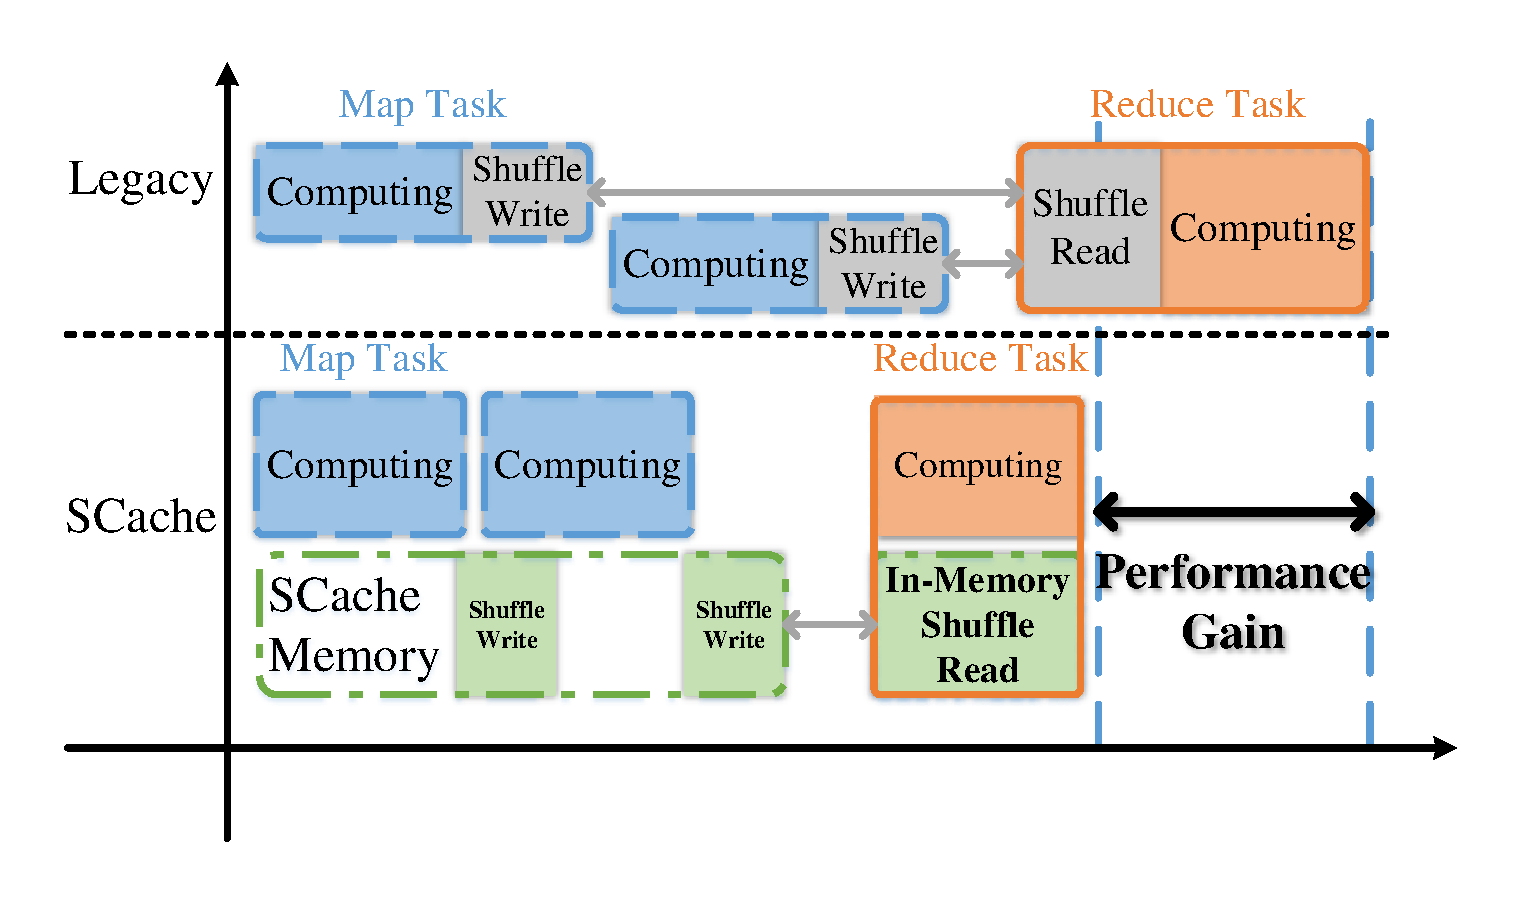
\includegraphics[width=\linewidth]{fig/workflow}
	\caption{Workflow Comparison between Legacy DAG Computing Frameworks and Frameworks with SCache}
	\label{fig:workflow}
	\vspace{-1em}
\end{figure}

Moreover, the shuffle read phase introduces all-to-all communication pattern across the network, and such network I/O procedure is also poorly coordinated.
Note that the shuffle read phase starts fetching data only after the corresponding reduce tasks start.
Meanwhile, the reduce tasks belonging to a same execution phase are scheduled at the same time by default. 
As a result, all the corresponding reduce tasks start fetching shuffle data almost simultaneously.
Such synchronized network communication causes a burst demand for network I/O, which in turn greatly enlarges the shuffle read completion time. 
To desynchronize the network communication, an intuitive way is to launch some tasks in the descendent stage earlier, such as "slow-start" from Hadoop MapReduce\cite{hadoop}. 
However, such early-start is by no means a panacea. 
\hlyellow{
This is because the early-start always introduces an extra early allocation of slot, which slows down the current stage execution.
}
% This is because although the reduce tasks can start fetching data earlier, the computation can only take place after all the data is ready. 

%In one word, existing solutions suffer from either inefficient use of network I/O, or a waste of computational resources (i.e., CPU and memory) caused by task pre-launching.

%For example, Apache Hadoop \cite{hadoop} provides an \emph{early start} mechanism that launches reduce tasks after a certain portion (5\% by default) of map tasks has completed, which is adopted in many of the recent works \cite{ihadoop, ishuffle, dynmr}.
% DAG computing framworks deriving from MapReduce \cite{mapreduce} contains a hard barrier between computing stages. The terminology of this barrier is \textit{shuffle}. Shuffle contains two parts on the connecting stages -- \textit{shuffle write} and \textit{shuffle read}. On the side of ancestor stages, \textit{shuffle write} is resoponsible for writing intermediate results to disk. On the side of descendant stage, \textit{shuffle read} fetches intermediate results from remote disks through network. Although highly optimized in other factors, the shuffle of framework is still primitive.  The coarse design of shuffle introduce a significiant performance overhead.
% % design inconsistent
% For instance, a MapReduce trace analysis from Facebook shows that shuffle accounts for 33\% JCT on average, up to 70\% in shuffle-heavy jobs \cite{managing}.
% shuffle operations
% three resource coordinate 不好
% 计算和I/O couple, why
% why disk, reason!!!, 不重视
% common problems

To make things worse, we note that the above deficiencies generally exist in most of the DAG computing frameworks. 
As a result, even we can effectively resolve the above deficiencies by modifying one framework, updating one application at a time is impractical given the sheer number of computing frameworks available today.

% The main defect of current shuffle design is coarse granularity of resource allocation during the task scheduling.
% Nearly all task scheduling algorithms in DAG frameworks use time slotted model. Specifically, when a task is launched, the framework offers it a bundle of resources (i.e. CPU and memory), which are dedicated to this task during the time in its "slot".
% But for a task, the resources demand changes during different phases. The computing phase is CPU and memory intensive. The shuffle, instead, is I/O intensive.
% As shown in the upper part of Figure \ref{fig:workflow}, this "slot" can be released until the map tasks finish \textit{shuffle write} on disk. And the "slot" is occupied when the reduce tasks begin to read shuffle data from remote nodes through network, which is presented as \textit{shuffle read}. This inconsistency between demands and allocation results in a severe resource underutilization, which slow down the framework.

% Another drawback of current shuffle is the synchronized shuffle read. When all the reduce tasks are scheduled, the shuffle fetch of each task starts almost simultaneously, which may cause congestion of network and delay the shuffle read. The straight forward way to avoid network burst is to start reduce tasks earlier. Apache Hadoop \cite{hadoop} provides a mechanism that schedules reduce tasks when a certain portion of map tasks completed. So that the shuffle delay can be mitigated. Other publications also purpose solutions to pre-schedule reduce tasks \cite{ihadoop, ishuffle, dynmr}. However this early scheduling of reduce tasks occupies new task slots, which degrades system performance. To this end, we proposed a question for this cross-frameworks issue, \textit{can we efficiently optimize shuffle without manually change every DAG framework?}




% 针对性的提出这三个点
% three resource coordinate 不好
% 计算和I/O couple, why
% why disk, reason, 不重视
% common problems
% 总起:普适性工具
% pre-fetch but not pre-execute
% byproduct: more balance
% memory instead of disk

% challenge point by point, inside the problem

Can we efficiently optimize the data shuffling without significantly changing every framework?
In this paper, we answer this question in the affirmative with S(huffle)Cache, an open source plug-in system which provides a shuffle-specific optimization for different DAG computing frameworks.
Specifically, SCache takes over the whole shuffle phase from the underlying framework by providing a cross-framework API for both shuffle write and read.
SCache's effectiveness lies in the following two key ideas.
First, SCache decouples the shuffle write and read from both map and reduce tasks.
Such decoupling effectively enables fine-grained resource management and better multiplexing between the computational and I/O resources.
\hlyellow{
In addition, SCache pre-schedules the reduce tasks \emph{without launching} them and pre-fetches the shuffle data for the reduce tasks.
Such pre-scheduling and pre-fetching effectively overlap the network transfer time, desynchronize the network operations, 
and avoid the extra early allocation of slots.
}
%In this paper, we introduce S(huffle)Cache, an plugin system to remove shuffle latency for DAG frameworks. SCache takes over the management of shuffle and I/O resources to acheive a fine granularity scheduling of tasks. In addition, SCache pre-schedules the reduce tasks without launching them and perform shuffle data pre-fetch to break the synchronization of shuffle fetch. In order to provide a general optimization for different DAG frameworks, SCache decouple the shuffle process from computing and  provide a cross-frameworks API for shuffle write and read.

The workflow of DAG framework with SCache is presented in Figure \ref{fig:workflow}. 
\hlyellow{
SCache hijacks the shuffle data of a map task in memory space. 
The disk operation is skipped and the slot is released after memory copy. 
The in-memory shuffle data is immediately pre-fetched through network after pre-scheduling of reduce tasks. 
The application-context-aware memory management caches the shuffle data in memory before the start of the reduce task.
By applying these optimizations, SCache can help the DAG framework achieve a significant performance gain. 
}

The main challenge to achieve this optimization is \textit{pre-scheduling reduce tasks without launching}. 
% It is not critical for the simple DAG computing such as Hadoop MapReduce \cite{mapreduce}. 
\hlyellow{
Firstly, the complexity of DAG can amplify the defects of na\"{i}ve scheduling schemes. 
In particular, randomly assigning reduce tasks might result in a collision of two heavy tasks on one node. 
This collision can aggravate data skew, thus hurting the performance. 
Secondly, pre-scheduling without launching violates the design of most frameworks that launch a task after scheduling.
To address the challenges, we propose a heuristic task pre-scheduling scheme with shuffle data prediction and a task co-scheduler} (Section \ref{opt}).

Another challenge is the \textit{in-memory data management}. 
To prevent shuffle data touching the disk, SCache leverages extra memory to store the shuffle data. 
However, the memory is a precious resource for DAG computing. 
To minimize the reserved memory while maximizing the performance gain, we propose two constraints: all-or-nothing and context-aware (Section \ref{memorymanage}).
%The memory management scheme follows these two contraints to switch shuffle data blocks on and off reserved memory.

We have implemented SCache and a customized Apache Spark \cite{apachespark}. 
The performance of SCache is evaluated with both simulations and testbed experiments on a 50-node Amazon EC2 cluster. 
We conduct basic test GroupByTest. 
We also evaluate Terasort \cite{spark-tera} benchmark and standard workloads like TPC-DS \cite{tpcds} for multi-tenant modeling. 
In a nutshell, SCache can eliminate explicit shuffle process by at most $89\%$ in varied application scenarios. 
More impressively, SCache reduces $~40\%$ of overall completion time of TPC-DS queries on average.


\section{Motivation}

In this section, we first study the typical shuffle characteristics (\ref{shuffle pattern}), and then spot the opportunities to achieve shuffle optmization (\ref{observation})
\subsection{Characteristic of Shuffle} \label{shuffle pattern}

In large scale data parallel computing, enormous datasets are partitioned into pieces to fit into the memory of single node.
Meanwhile, complicated application procedures are divided into steps. The succeeding steps take the output of ancestors as computation input. Shuffle occurs when each successor needs 
part of data from all ancestors' output. It is designed to achieve an all-to-all data blocks transfer in cluster. It exists in both MapReduce models and DAG computation models.
For clear illustration, we define those computing on each partition of data in one step as a \textit{task}. 
Those tasks that generate shuffle outputs are called as \textit{map} tasks, and tasks consuming shuffle outputs are called as \textit{reduce} tasks.
% Note that one task may have both shuffle data generation and consumption in modern DAG framework. These tasks contain characteristic of both map task and reduce task. But these tasks won't change the behavior of shuffle. To avoid ambiguity, in the following paper, we will only use term of map task to represent those who produce shuffle output, and reduce task to represent those who consume shuffle output.

\textbf{Overview of shuffle process}. As shown in Figure \ref{fig:shuffle_process}, shuffle data is produced by \textit{data partition}. For \textit{data partition}, each map task will partition the result data (key, value pair) after execution ("Execution" block in Figure \ref{fig:shuffle_process}) into several buckets according to the partition function.
The total number of buckets equals to the number of tasks in the next step. 
Shuffle itself is dedicated to achieve all-to-all \textit{data transfer}.
It can be further split into two parts: \textit{shuffle write} and \textit{shuffle read}. Shuffle write starts after data partition ("Data Partition" block in Figure \ref{fig:shuffle_process}) of map tasks. 
All the partitioned shuffle output data will be written into local persistent storage for fault tolerance \cite{mapreduce, spark} during shuffle write.
Shuffle read starts fetching data that belong to their corresponding partitions from both remote nodes and local storage at the beginning of reduce tasks.

%In short, shuffle is loosely coupled with application context and it's I/O intensive.

\textbf{Impact of shuffle process}. Shuffle process is I/O intensive, which might can introduce a significant latency to the application. Reports show that 60\% of MapReduce jobs at Yahoo!
and 20\% at Facebook are shuffle intensive workloads \cite{shufflewatcher}. For those shuffle intensive jobs, the shuffle latency may even dominate Job Completion Time (JCT). 
For instance, a MapReduce trace analysis from Facebook shows that shuffle accounts for 33\% JCT on average, up to 70\% in shuffle intensive jobs \cite{managing}.
% Besides, the completion time of shuffle correlates with the performance of storage devices, network and even applications. 
% This variation may bring a huge challenge for operators to find the correct configuration of the DAG framework.
\begin{figure}
	\centering
	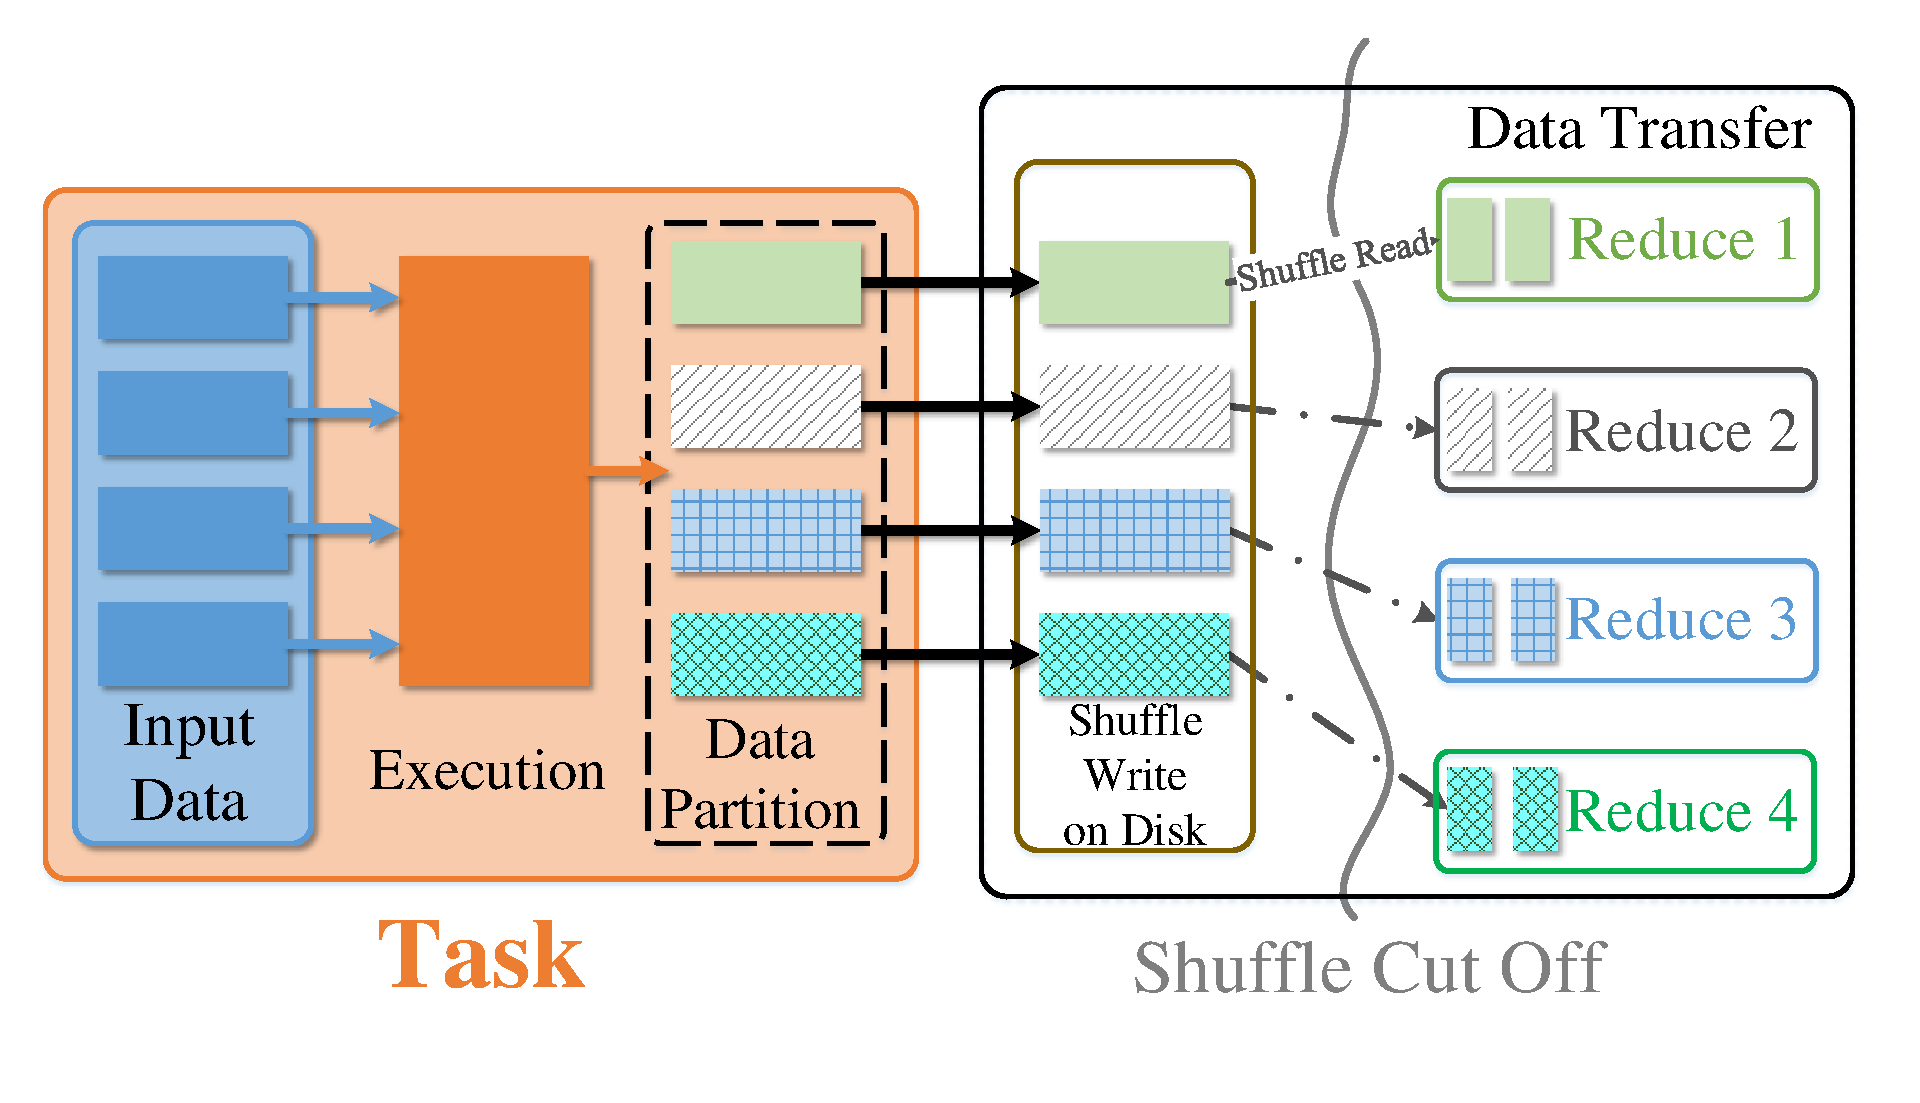
\includegraphics[width=\linewidth]{fig/shuffle_process}
	\caption{Shuffle Overview}
	\label{fig:shuffle_process}
\end{figure}

\subsection{Observations} \label{observation}
Of course, shuffle is unavoidable in a DAG computing process. But can we mitigate or even remove the overhead of shuffle? To find the answers, we run some typical Spark applications in a 5-node EC2 cluster with \texttt{m4.xlarge}. We then measure the CPU utilization, I/O throughput and tasks execution information of each node. Here we present the trace of one node running Spark \textit{GroupByTest} in Figure \ref{fig:util} as an example. This job has 2 rounds of tasks for each node. 
We have marked out the \textit{execution} phase as from the launch time of the first task to the execution finish timestamp of the last one. The \textit{shuffle write} phase is marked from the timestamp of the beginning of the first partitioned data write. The \textit{shuffle read and execution} phase is marked from the start of the first reduce launch timestamp.

Figure \ref{fig:util} reveals the performance information of two stages that are connected by shuffle. By analyzing the trace combing with Spark source code \cite{sparksource}, we propose the following observations. 
% \begin{figure*}
% 	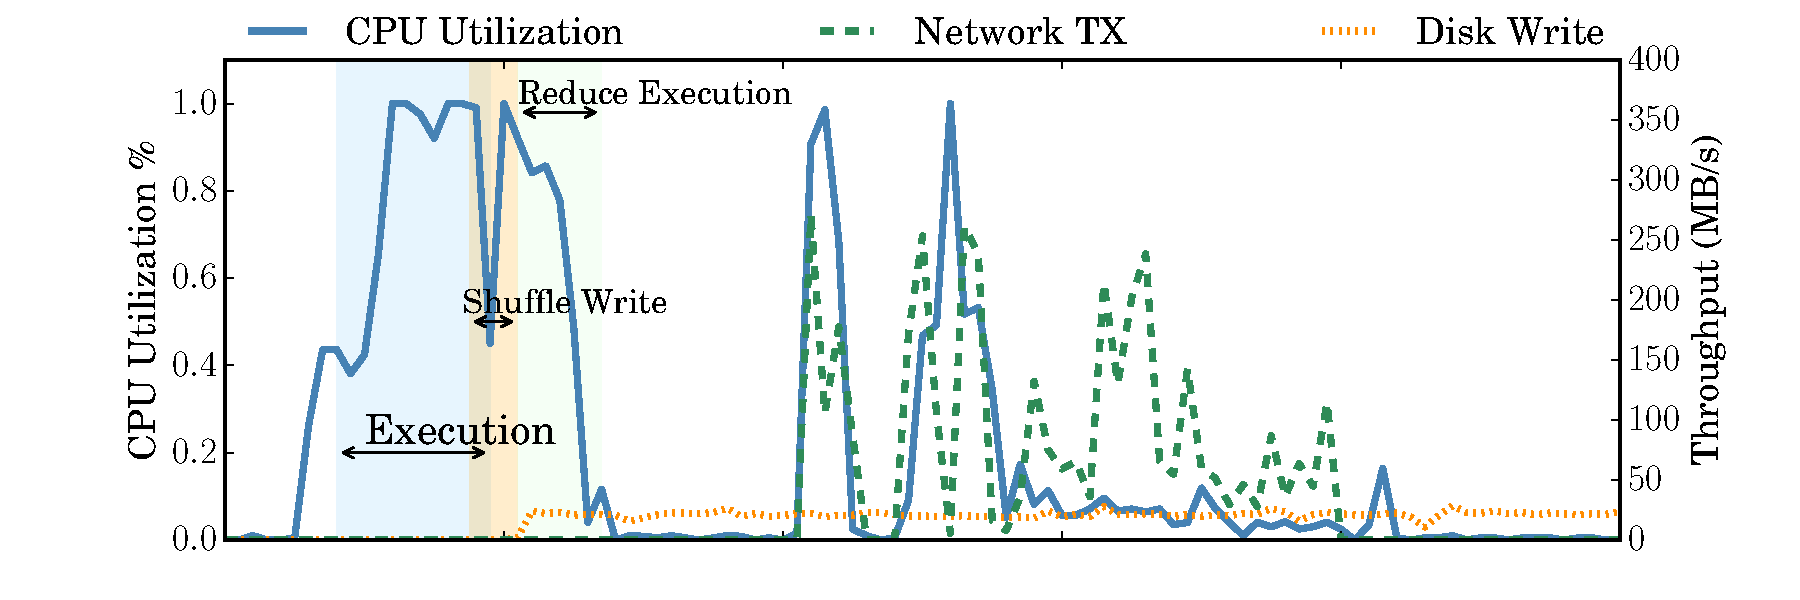
\includegraphics[width=\textwidth]{fig/util}
% 	\caption{CPU utiliazation and I/O throughput of a node during a Spark single shuffle application}
% 	\label{fig:util}
% \end{figure*}

\begin{figure}
	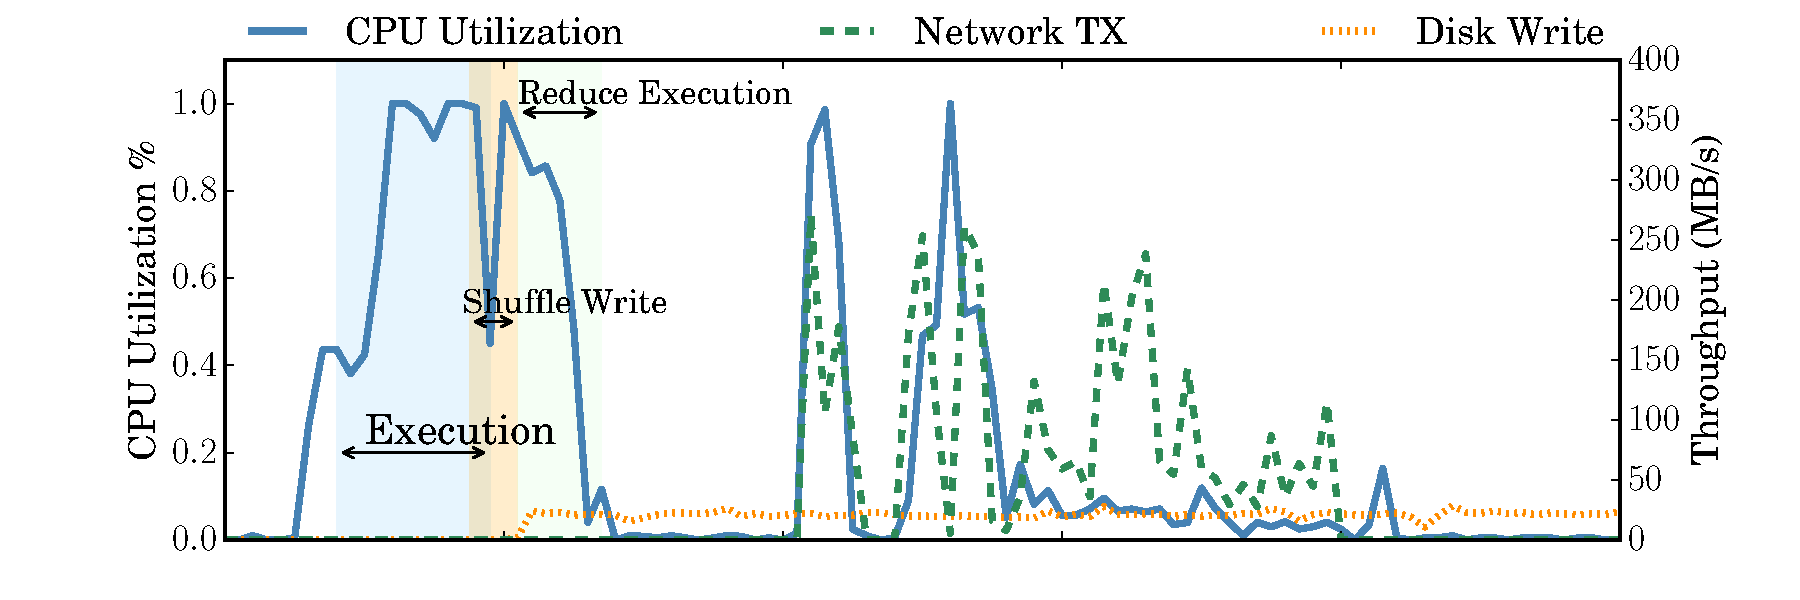
\includegraphics[width=\linewidth]{fig/util}
	\caption{CPU utilization and I/O throughput of a node during a Spark single shuffle application}
	\label{fig:util}
\end{figure}

\subsubsection{Coarse Granularity Resource Allocation}
In general, CPU and memory are bounded with a schedule slot in DAG resource scheduler. When a task is scheduled to a slot, it will not release the until the end of the task. In Figure \ref{fig:util}, the resource of Spark executor will be released at the ending of \textit{shuffle write}. On the reduce side, though in the context of Spark, the reduce task can do computation while fetching data, the transfer of first few blocks may still introduce an explict I/O delay. On the other hand, shuffle is an I/O intensive job without involving CPU. Both \textit{shuffle write} and \textit{shuffle read} occupy the slot without using CPU. The current coarse slot --- task mapping results in an inconsistency between resource demands and slot allocation, which further decrease the resource utilization. To break this inconsistency, a finer granularity resource allocation scheme must be provided.

\subsubsection{Synchronized Shuffle Read}
Combining with traces from other nodes, we find that almost all reduce tasks start \textit{shuffle read} simultaneously (i.e. The rising network utilization during \textit{shuffle read and execution} in Figure \ref{fig:util}). The synchronized \textit{shuffle read} requests cause a burst of network traffic. As shown in Figure \ref{fig:util}, the data transfer stresses on network bandwidth, which may result in network congestion among the cluster. This bursty demands of network bandwidth might delay the \textit{shuffle read} and hurt the performance of reduce stage. The previous work \cite{coflow, managing} also prove that the network transfer can introduce significant overhead in DAG computing.

\subsubsection{Multi-round Tasks Execution}\label{multi}
Both experience and DAG framework manuals recommend that multi-round execution of each stage will benefit the performance of applications.
For example, Hadoop MapReduce Tutorial  \cite{hadooptutorial} suggests that \textit{10-100 maps per-node} and \textit{0.95 or 1.75 $\times$ no. of nodes $\times$ no. of maximum container per node} seem to be the right level of parallelism. Spark Configuration also recommends 2-3 tasks per CPU core in the cluster \cite{sparkconf}.
In Figure \ref{fig:util} we also run two rounds of tasks to process data of about $70$GB. As shown in Figure \ref{fig:util}, during the map stage, the network is idle (i.e. Network utilization during \textit{execution} and \textit{shuffle write}). Since the shuffle data becomes available as soon as the execution of one map task is finished, if the destination of the shuffle output of each task can be known in priori, the property of multi-round can be leveraged to do \textit{shuffle read} ahead of reduce stage.


\subsubsection{Unefficient Persistent Storage Operation}
When we look into the detail I/O operations of shuffle, we find that the operations on persistent storage of shuffle are unefficient. There are at least two persistent storage operations for each shuffle data block. At first, Spark will write shuffle data to the persistent storage after map task execution(i.e. \textit{Shuffle Write} in Figure \ref{fig:util}). During the \textit{shuffle read}, Spark will then read shuffle data from remote and local presistent storage, which is the second operation. The persistence of shuffle data was designed for fault tolerance. But we believe it's not necessary for today's cluster. Recall that shuffle data only exist in a short time scale. But the Mean Time To Failure(MTTF) for a server is counted in the scale of year \cite{tachyon}, which is exponential comparing with the duration of a shuffle. In addition, the capacity of memory and network has been increasing rapidly in recent years. As a result, numbers of memory based distributed storage system have been proposed \cite{memcached, tachyon, ramcloud}. On the other hand, the size of shuffle data is relatively small. For example, shuffle size of Spark Terasort \cite{spark-tera} is less than 25\% of input data. The data reported in  \cite{makingsense} also shows that the amount of data shuffled is less than input data, by as much as 10\%-20\%. We argue that removing persistent storage and using memory to achieve shuffle fault tolerance is feasible and efficient.

Based on these observations, it is straightforward to come up with an optimization that uses memory to store the shuffle data and start \textit{shuffle read} ahead of reduce stage to overlap the I/O operations in \textit{multi-round} of DAG computing. To achieve this optimization:
\begin{itemize}
	\item Shuffle should be taken over to provide a fine granularity scheduling scheme.
	\item Reduce tasks should be pre-scheduled without launching to achieve shuffle data pre-fetch.
	\item Shuffle process should be decoupled to provide a cross-framework optimization
\end{itemize} 
In the following section, we elaborate the methodologies to achieve three design goals.

\section{Shuffle Optimization}
In this section, we present the detailed methodologies to achieve three design goals. The memory copy is used to decouple shuffle from execution. Shuffle data is pre-fetched without tasks launching with the heuristic MinHeap pre-scheduling scheme. And all shuffle data is managed outside DAG framework by SCache to provide a universal cross-framework optimization.
We choose Spark \cite{apachespark} as the representative of DAG computing framework to implement our optimization.

\begin{figure}
	\centering
	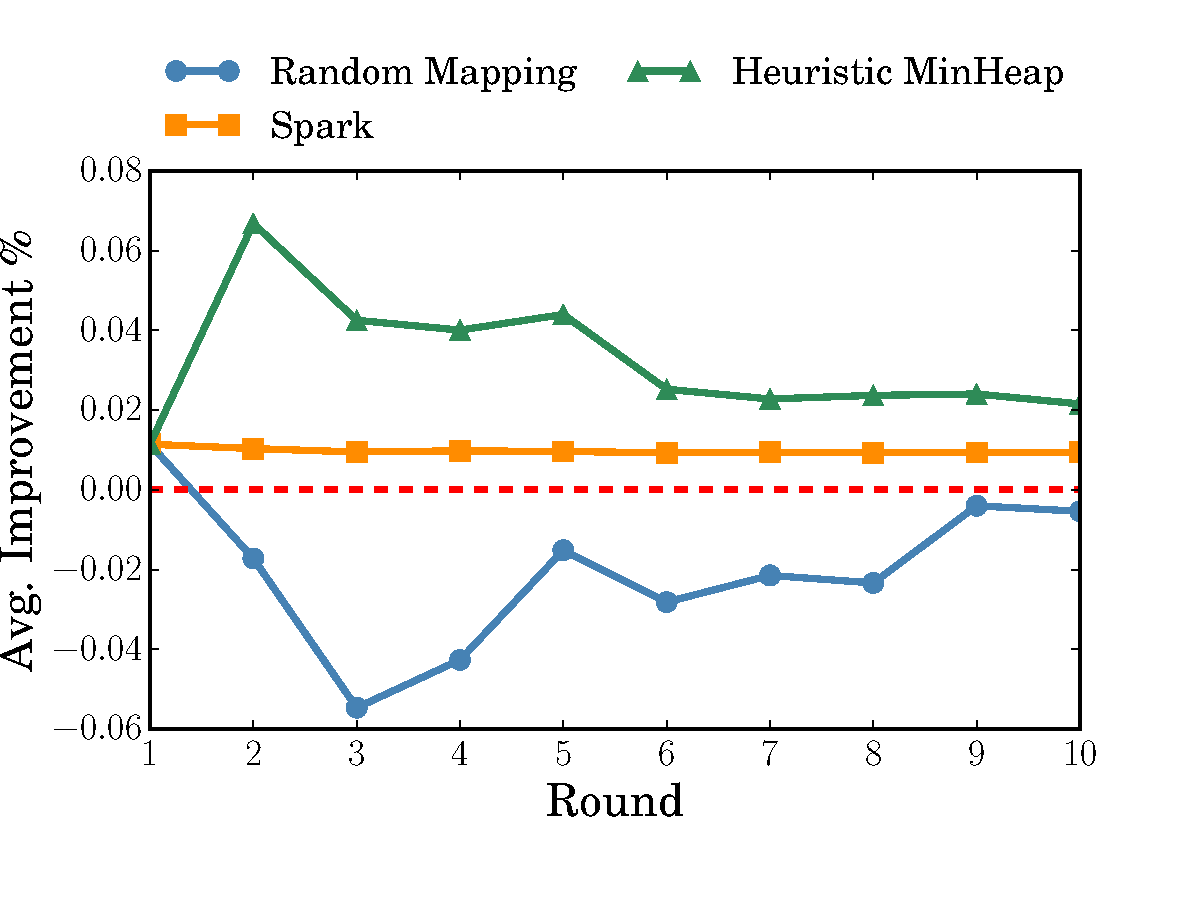
\includegraphics[width=0.9\linewidth]{fig/sim}
	\caption{Stage Completion Time Improvement of OpenCloud Trace}
	\label{fig:sim}
\end{figure}

\subsection{Decouple Shuffle from Execution}
In map tasks the partitioner takes a set of key-value pairs as input and calculates the partition number of a key-value pair by applying pre-defined the partition function to the key. After that, it stores the key-value pair in the corresponding data blocks. Each of the block contains the key-value pairs for one reduce partition. At last, blocks will be flushed to disk. The decoupling starts before data flushing. To avoid blocking the slot by disk write, we use memory copy to hijack shuffle data from Spark executor's JVM space. By doing this, a slot can be released as soon as it finishes CPU intensive computing. The pre-scheduling and pre-fetch starts when the collected shuffle data exceeds the threshold.

On the reduce side, shuffle read is decoupled by pre-fetching shuffle data to local SCache client after pre-scheduling before reduce tasks start.

To this end, all I/O operations are managed outside of the DAG framework, and the slot is occupied only by the CPU intensive phases of task.

\begin{figure}
	\centering
	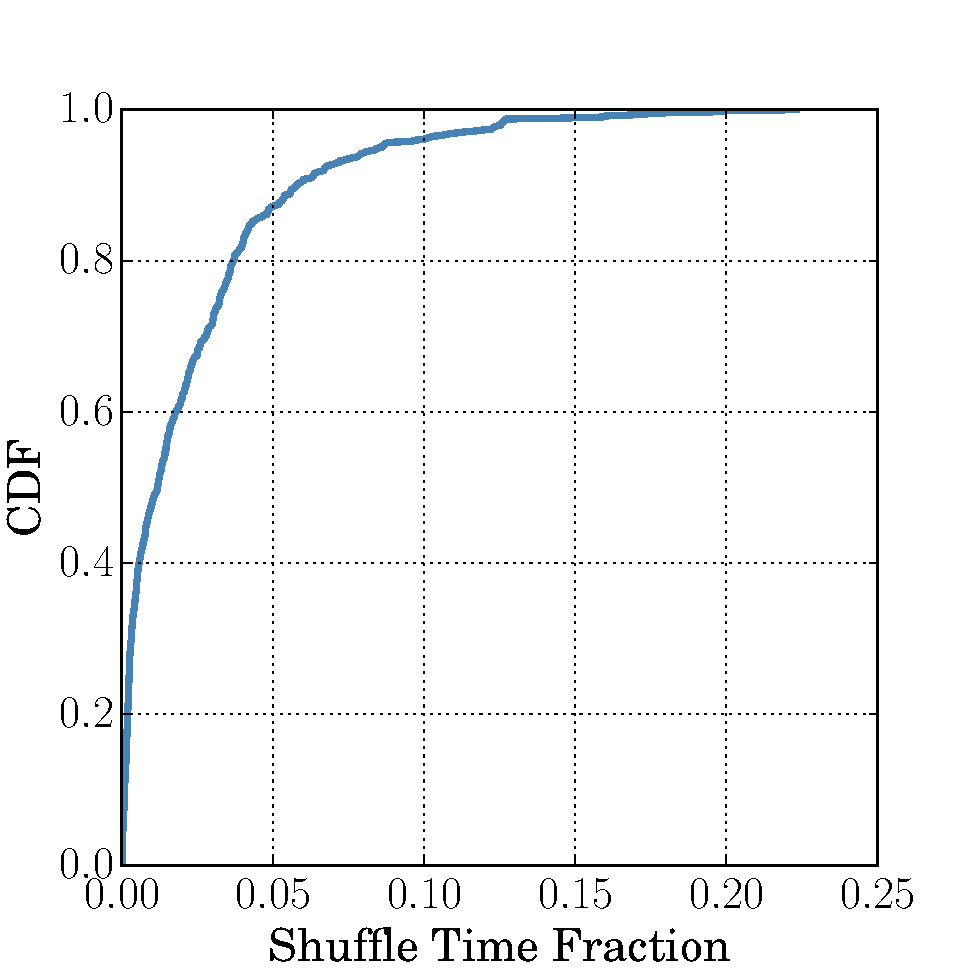
\includegraphics[width=0.75\linewidth]{fig/reduce_cdf}
	\caption{Shuffle Time Fraction CDF of OpenCloud Trace}
	\label{fig:cdf}
\end{figure}

\subsection{Pre-schedule with Application Context}
The main challenge toward the optimization is how to pre-schedule the reduce tasks without launching. The task --- node mapping is not determined until tasks are scheduled by scheduler of DAG framework. But as soon as they are scheduled, slots will be occupied to launch them. On the other hand, shuffle data cannot be pre-fetched without knowing the task --- node mapping.
To get rid of this dilemma, we propose a co-scheduling scheme. That is, the task --- node mapping is established ahead of DAG framework scheduler, and then enforce the mapping results to DAG scheduler while doing the real scheduling.

We use traces from OpenCloud \cite{opencloudtrace} for the simulation to evaluate the impact of different pre-scheduling schemes. The baseline (red dot line in Figure \ref{fig:sim}) is the stage completion time under Spark default scheduling algorithm. And then we remove the shuffle read time of each task, and do the simulation under three different schemes: random mapping, Spark FIFO, and our heuristic MinHeap.

% We explore several pre-scheduling schemes in different scenarios, and evaluate the performance calculating the improvement of reduce tasks completion time with trace of OpenCloud \cite{opencloudtrace}. We first emulate the scheduling algorithm of Spark to schedule the reduce tasks of one job, and take the bottleneck of the task set as the completion time. Then we remove the shuffle read time as the assumption of shuffle data pre-fetch and emulate under different schemes. The result is shown in \ref{fig:sim}.
% \begin{figure*}
% 	\centering
% 	\begin{minipage}{0.34\linewidth}
% 		\begin{figure}[H]
% 			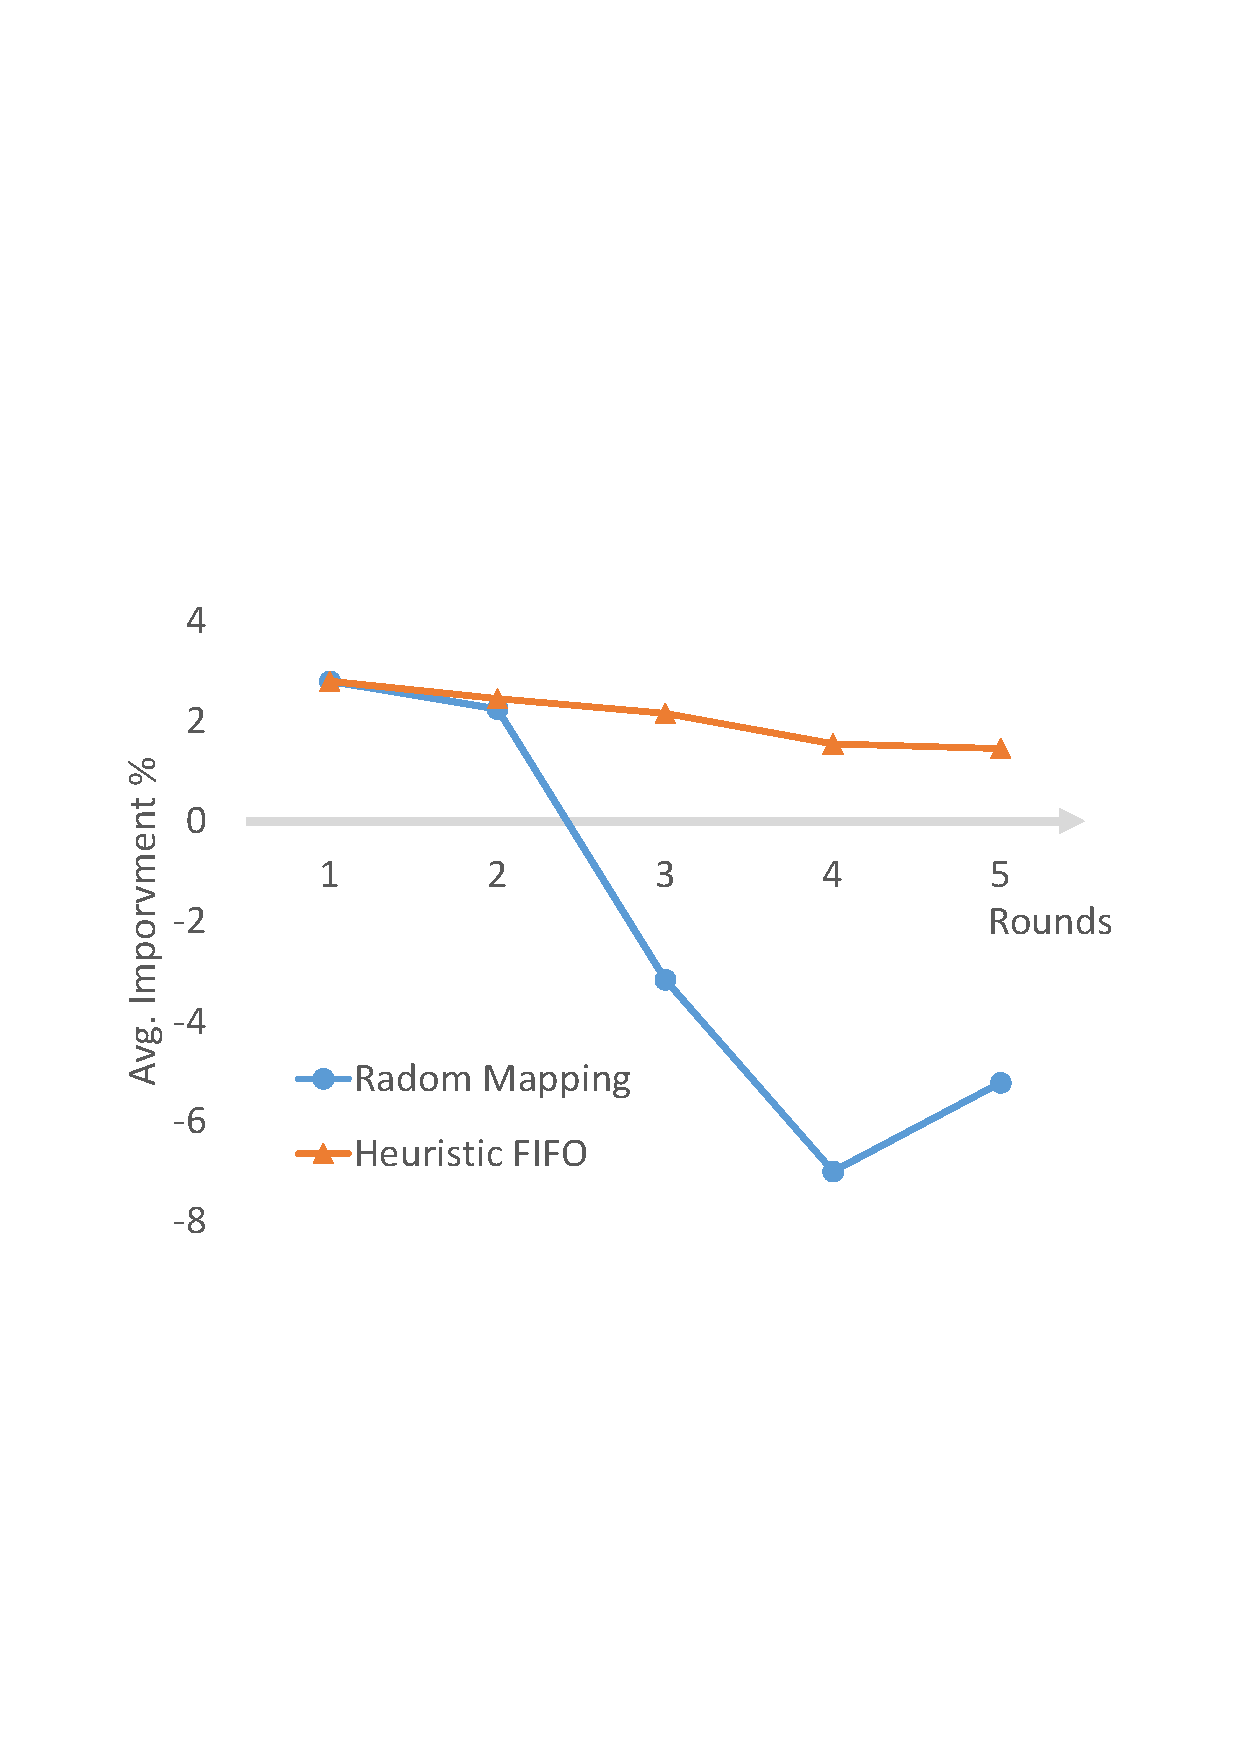
\includegraphics[width=\textwidth]{fig/shuffle_size}
% 			\caption{Shuffle Size Comparing with Input Size}
% 			\label{fig:shuffle_size}
% 		\end{figure}
% 	\end{minipage}
% 	\begin{minipage}{0.65\linewidth}
% 		\begin{figure}[H]
% 			\begin{subfigure}{0.5\textwidth}
% 				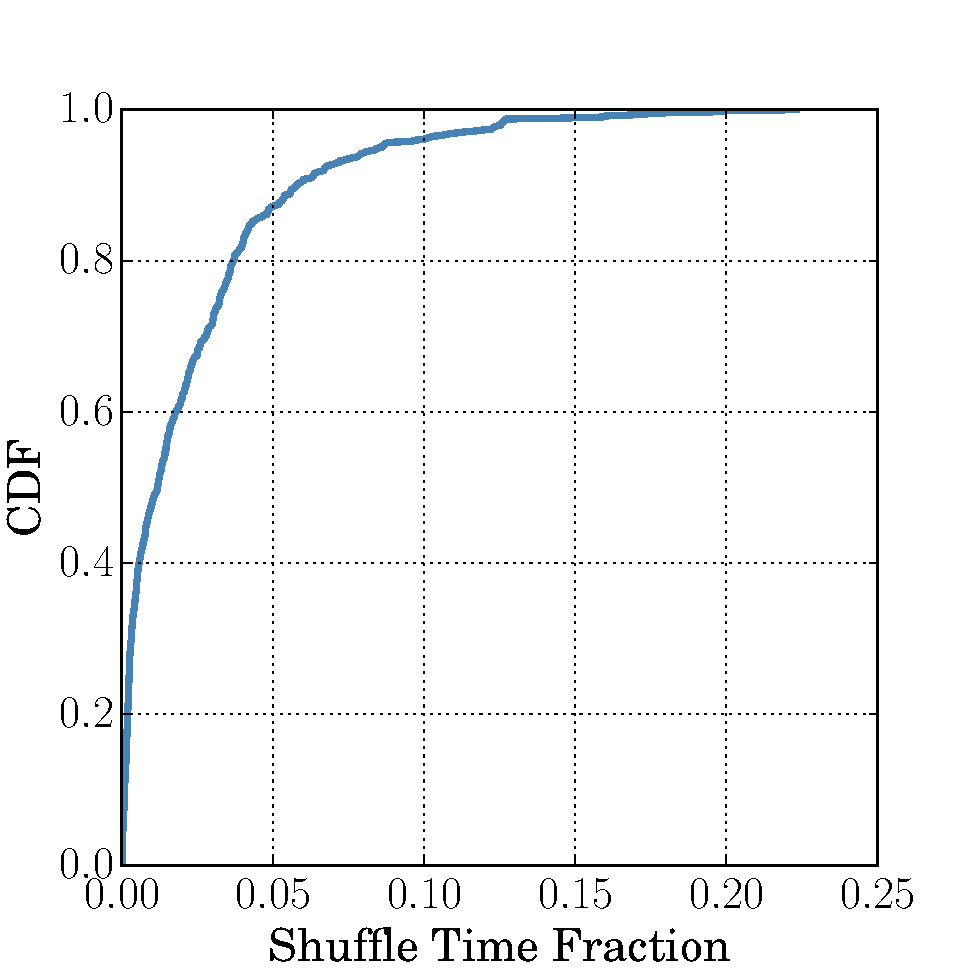
\includegraphics[width=\linewidth]{fig/reduce_cdf}
% 				\caption{Shuffle Time Fraction CDF}
% 				\label{fig:cdf}
% 			\end{subfigure}	
% 			\begin{subfigure}{0.5\textwidth}
% 				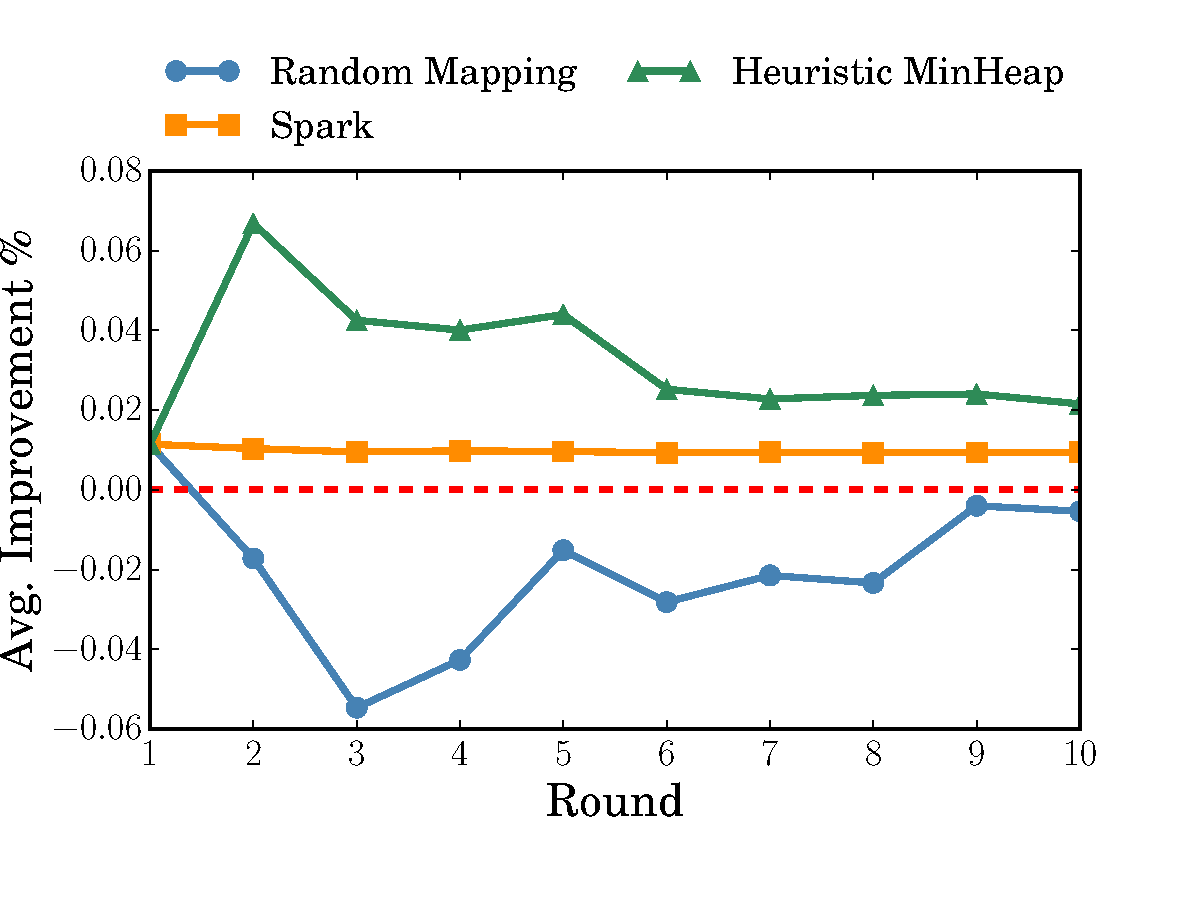
\includegraphics[width=\linewidth]{fig/sim}
% 				\caption{Stage Completion Time Improvement}
% 				\label{fig:sim}
% 			\end{subfigure}	
% 			\caption{Emulate Result of OpenCloud Trace}
% 		\end{figure}
% 	\end{minipage}
% \end{figure*}
% \begin{figure}



Note that most of the traces from OpenCloud is shuffle-light workload as shown in Figure \ref{fig:cdf}. The average shuffle read time is 2.3\% of total reduce completion time.

\subsubsection{Failure of Random Mapping}\label{randomassign}
The simplest way of pre-scheduling is mapping tasks to different nodes randomly. It only guarantees that each node run same number of tasks. As shown in Figure \ref{fig:sim}, Random mapping works well when there is only one round of tasks. But the performance collapses as the round number grows. It is because that data skew commonly exists in data-parallel computing \cite{skewtune, reining, gufler2012load}. Several heavy tasks might be assigned on the same node. This collision then slows down the whole stage and makes the performance even worse than the baseline. In addition, randomly assigned tasks also ignore the data locality between shuffle map output and shuffle reduce input, which might introduce extra network traffic in cluster.


\subsubsection{Shuffle Output Prediction}\label{shuffleprediction}
The failure of random mapping was obviously caused by application context (e.g. shuffle data size) unawareness. Note that the optimal schedule decision can be made under the awareness of shuffle dependencies number, partition number and shuffle size for each partition. The first two of them can be easily extracted from DAG information. To achieve a better scheduling result, the shuffle size for each partition should be predicted during the initial phase of map tasks.

According to the DAG computing process, the shuffle size of each reduce task is decided by input data, map task computation, and hash partitioner. Each map task produces a data block for each reduce task. The size of each reduce partition can be calculated $reduceSize_i = \sum_{j=0}^{m} {BlockSize_{ji}}$ ($m$ is the number of map tasks). $BlockSize_{ji}$ represents the size of block which is produced by map $task_j$ for reduce $task_i$ (e.g., block `1-1' in Figure \ref{fig:shuffle}).

For Hadoop MapReduce, the $BlockSize_{ji}$ can be predicted with decent accuracy by liner regression model based on observation that the ratio of map output size and input size is invariant given the same job configuration \cite{ishuffle, predict}.

But the sophisticated DAG computing framework like Spark introduces more uncertainties. For instance, the reduce stage in Spark has more tasks than Hadoop MapReduce. More importantly, the customized partitioner might bring huge inconsistency between observed map output blocks distribution and the final reduce input distribution as presented in Figure \ref{fig:dis}. We use different datasets with different partitioners and normalize three sets of data to $0-1$ to fit in one figure. In Figure \ref{fig:hash_pre}, we use a random input dataset with the hash partitioner. In Figure \ref{fig:range_pre_sample}, we use a skew dataset with the range partitioner of Spark \cite{sparksource}.
The observed map outputs are randomly picked. As we can see, in hash partitioner, the distribution of observed map output is close to the final reduce input distribution. The prediction results also turn out to be good. However, the huge inconsistency between final reduce distribution and observed distribution results in a deviation in linear regression model.
% Several map outputs (marked as Map Output in Figure \ref{fig:shuffle}) are picked as observation objects to train the model and than predict the final reduce distribution.

\begin{equation}
\label{equationsample}
\begin{aligned}
	BlockSize_{ji} &= {{InputSize_j \times \frac{sample_i}{s \times p}}} \\
	sample_i &= \text{number of samples for $reduce_i$}
\end{aligned}
\end{equation}

To handle this inconsistency, we introduce another methodology named weighted reservoir sampling. The classic reservoir sampling is designed for randomly choosing \textit{k} samples from \textit{n} items, where \textit{n} is either a very large or an unknown number \cite{reservoir}. For each partition of map task, we use reservoir sampling to randomly pick $s \times p$ of samples, where $p$ is the number of reduce tasks and $s$ is a tunable number. The number of input data partition and reduce tasks can be easily obtained from the DAG information. In Figure \ref{fig:range_pre_sample}, we set $s$ equals $3$. After that, the map function is called locally to process the sampled data (\textit{sampling} in Figure \ref{fig:shuffle}). The final sampling outputs are collected with the input size of each map partition which is used as weight for each set of sample.

As we can see in Figure \ref{fig:range_pre_sample}, the result of sampling prediction is much better even in a very skew scenario. The variance of the normalized between sampling prediction and reduce distribution is because the standard deviation of the prediction result is relatively small compared to the average prediction size, which is $0.0015$ in this example. Figure \ref{fig:prediction_relative_error} further proves that the sampling prediction can provide precise result even in the dimension of absolute shuffle partition size. On the opposite, the result of linear regression comes out with huge relative error.

However, sampling prediction trade accuracy with extra overhead in DAG computing process. Though in most cases, the overhead is acceptable, the sampling prediction will be triggered only when the range partitioner or customized non-hash partitioner occurs. We will show the overhead in the Section \ref{evaluation}.

During the phase of shuffle output prediction, the composition of each reduce partition is calculated as well. We define $prob_i$ as

\begin{equation}
\label{equationprob}
\begin{aligned}
	prob_i &= \max_{0 \leq j \leq m} \frac{BlockSize_{ji}}{reduceSize_i} \\
    m &= \text{number of map tasks}
\end{aligned}
\end{equation}

This parameter is used to achieve a better locality while performing shuffle scheduling.

\subsubsection{Heuristic MinHeap Scheduling}\label{h-minheap}
In order to achieve the uniform load on each node while reducing the network traffic, we present a heuristic MinHeap scheduling algorithm (\ref{hminheap}) for single shuffle.  
As for the input of $SCHEDULE$ function in Algorithm \ref{hminheap}, $m$ is the partition number of input data; $h$ is the array of nodes ID in cluster; $p\_reduces$ is the predicted reduce matrix. Each row in $p\_reduces$ contains $rid$ as reduce partition ID; $size$ as predicted size of this partition; $prob$ as the maximum composition portion of reduce data; $host\_id$ as the node ID that produces the maximum portion of reduce data, and $assigned\_id$ as the node ID assigned by Algorithm \ref{hminheap}. As for $M$, it is consists $host\_id$, an array of $reduce$ scheduled on this node and the $size$ of them.

\begin{minipage}{\columnwidth}
\begin{algorithm}[H]
\caption{Heuristic MinHeap Scheduling for Single Shuffle}
\label{hminheap}
	\begin{algorithmic}[1]
	\small
	\Procedure{schedule}{$m, h, p\_reduces$}
		\State $R\gets$ sort $p\_reduces$ by size in descending order
		\State $M\gets$ min-heap $\left\{ host\_id \rightarrow \left( \left[ reduces \right], size \right) \right\}$
		\State $idx\gets$ len$\left(R\right) - 1$
		\While{$idx \geq 0$}
		\Comment{Schedule reduces by MinHeap}
		\State $M\left[0\right].size \mathrel{+}= R\left[idx\right].size$
		\State $M\left[0\right].reduces.append\left(R\left[idx\right]\right)$
		\State $R\left[idx\right].assigned\_host \gets M \left[0\right].host\_id$
		\State Sift down $M\left[0\right]$ by $size$
		\State $idx\gets idx-1$
		\EndWhile
		\State $max\gets$ maximum size in $M$
		\State Convert $M$ to mapping $\left\{ host\_id \rightarrow \left( \left[ rid\_arr \right], size \right) \right\}$
		\ForAll{$reduce$ in $R$}
		\Comment{Heuristic swap by locality}
			\If{$reduce.assigned\_id \neq reduce.host\_id$}
				\State $p\gets reduce.prob$
				\State $norm\gets \left(p-1/m\right)/\left(1-1/m\right)/10$
				\State $upper\_bound \gets \left(1 + norm\right) \times max$
				\State SWAP\_TASKS$\left(M, reduce, upper\_bound\right)$
			\EndIf
		\EndFor
		% \Comment{$m$ is the number of input data}
		% \Comment{$r$ is partition number of reduces}
		% \Comment{$hosts$ is array of (hostid, partitionids[], size)}
		% \Comment{$c$ is $r*m$ array of composition data}
		% \Comment{$pSize$ is $r$ size array of predicted size of reduces}
		\Return $M$
	\EndProcedure
	\Procedure{swap\_tasks}{$M, reduce, upper\_bound$}
		\State $reduces \gets M\left[reduce.host\_id\right].reduce$	
		\State $candidates \gets$ Select from $reduces$ that $assigned\_id \neq host\_id$ \textbf{and} total size closest to $reduce.size$
		\State $\Delta size \gets sizeOf\left(candidates\right) - reduce.size$
		\State $size\_host \gets M\left[reduce.host\_id\right].size - \Delta size$
		\State $size\_assigned \gets M\left[reduce.assigned\_id\right].size + \Delta size$
		\If{$size\_host\leq upper\_bound$ \textbf{and} \\
			\qquad \; $size\_assigned\leq upper\_bound$}
			\State Swap $candidates$ and $reduce$
			\State Update $size$ in $M$
			\State Update $assigned\_host$ in $candidates$ and $reduce$
		\EndIf
	\EndProcedure
	\end{algorithmic}
\end{algorithm}
\end{minipage}


This algorithm can be divided into two rounds. In the first round (i.e., the first $while$ in $SCHEDULE$), the reduce tasks are first sorted by size in a descending order. For hosts, we use a min-heap to maintain the priority by size of assigned tasks. So that the tasks can be distributed evenly in the cluster.
% After the scheduling, the completion time of reduce stage is close to the optimal. \textcolor{red}{may need to add math prove between this and optimal}.
In the second round, the task --- node mapping will be adjusted according to the locality. 
The $SWAP_TASKS$ will only be trigged when the $host\_id$ of a reduce task is not equal the $assigned\_id$.
The closer $prob$ is to $1/m$, the more evenly this reduce partition is produced in cluster. For a task which contains at most $prob$ data from $host$, the normalized probability $norm$ is calculated as a bound of performance degradation. We set the $upper\_bound$ of performance degradation to be the 10\% slower than the origin (in extreme skew scenarios). This normalization can ensure that more performance would be traded when the locality level increases. 
Inside the $SWAP\_TASKS$, tasks will be selected and swapped without exceeding the $upper\_bound$ of each host. 
Unlike the na\"{i}ve Spark scheduling algorithm, these information helps the scheduler make a more balanced task --- node mapping, which accelerates the reduce stage. This is the by-product optimization harvested from shuffle size prediction.

We use the OpenCloud \cite{opencloudtrace} trace to evaluate Heuristic MinHeap. Without swapping, the Heuristic MinHeap can achieve a better performance improvement (average 5.7\%) than the default Spark FIFO scheduling algorithm (average 2.7\%).

% In the case of extreme skew scenario, such as Figure \ref{fig:range_pre_sample}, Heuristic MinHeap trades about 0.05\% percent of stage completion time for 99\% reduction of shuffle data transmission through network by heuristicly swapping tasks.

\begin{figure}
	\centering
	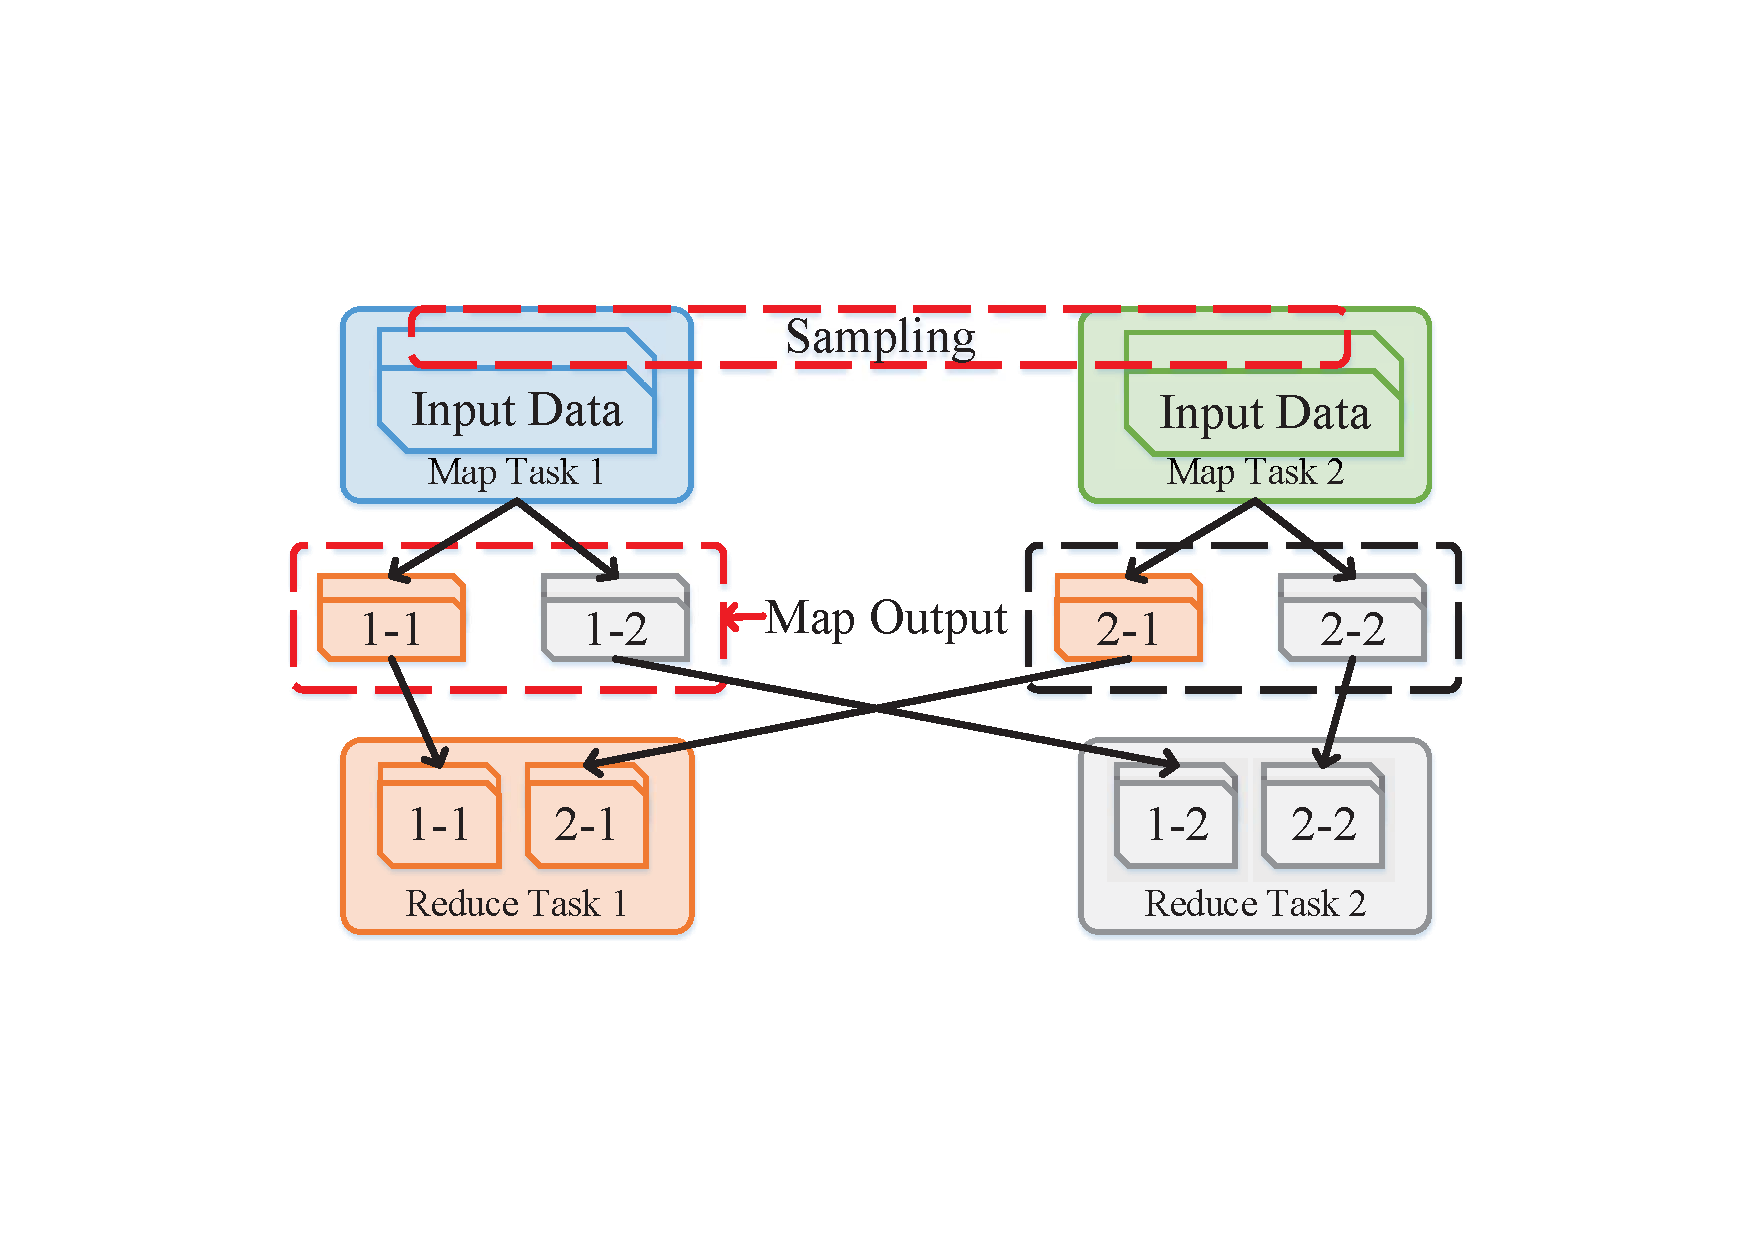
\includegraphics[width=0.9\linewidth]{fig/shuffle}
	\caption{Shuffle Data Prediction}
	\label{fig:shuffle}
\end{figure}

\begin{figure*}
	\centering
	\begin{subfigure}[b]{0.32\linewidth}
		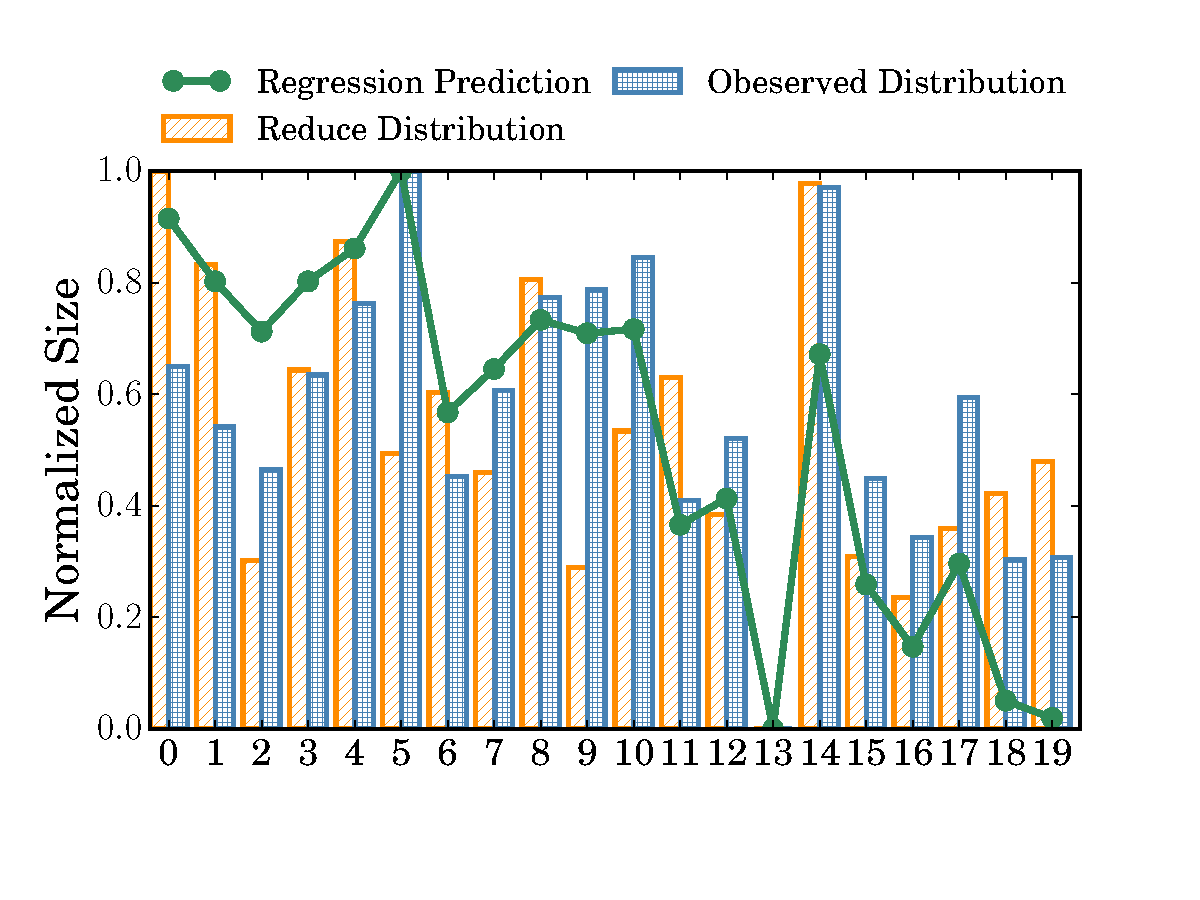
\includegraphics[width=\linewidth]{fig/hash_pre}
		\caption{Linear Regression Prediction of Hash Partitioner}
		\label{fig:hash_pre}
	\end{subfigure}
	\begin{subfigure}[b]{0.32\linewidth}
		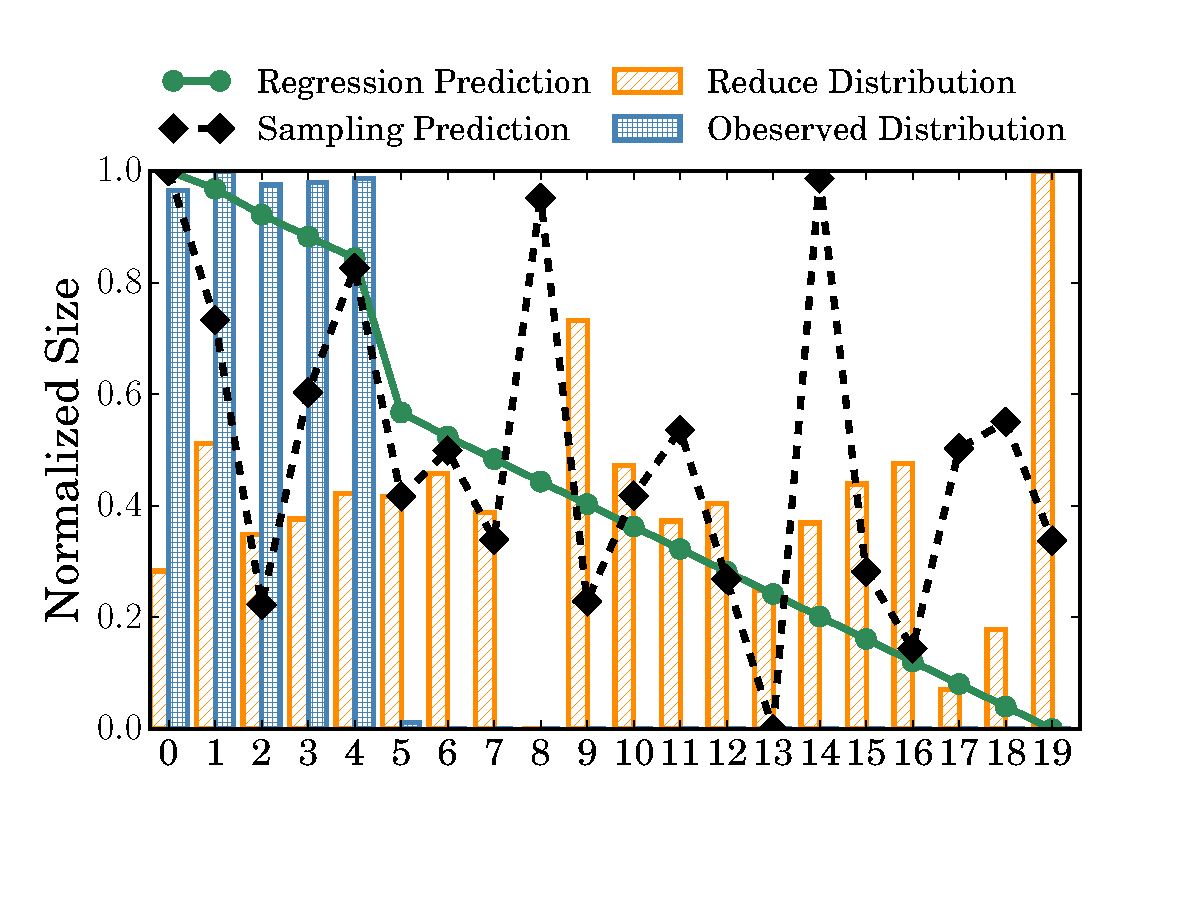
\includegraphics[width=\linewidth]{fig/range_pre_sample}
		\caption{Linear Regression and Sampling Prediction of Range Partitioner}
		\label{fig:range_pre_sample}
	\end{subfigure}
	\begin{subfigure}[b]{0.32\linewidth}
		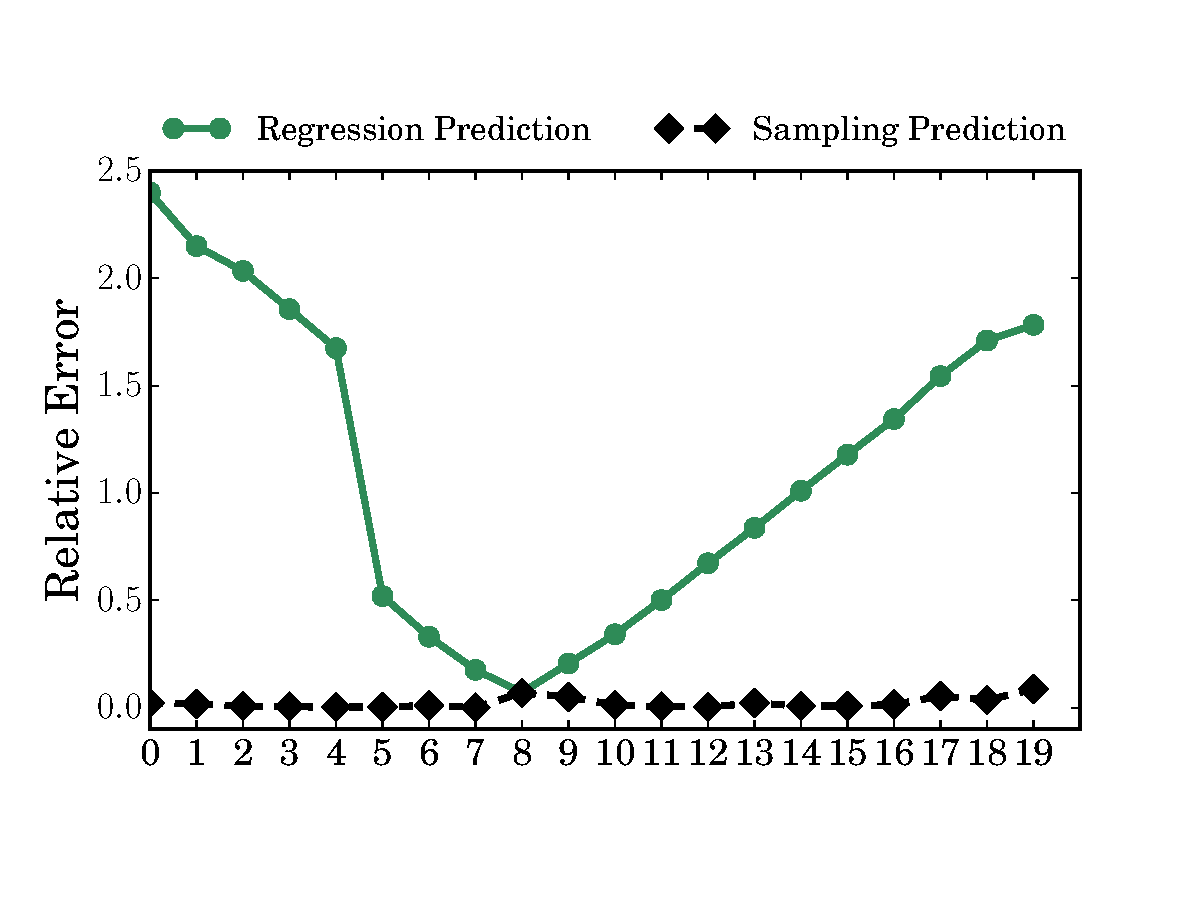
\includegraphics[width=\linewidth]{fig/prediction_relative_error}
		\caption{Prediction Relative Error of Range Partitioner}
		\label{fig:prediction_relative_error}
	\end{subfigure}
	\caption{Reduction Distribution Prediction}
	\label{fig:dis}
\end{figure*}

\subsubsection{Cope with Multiple Shuffles}
Unlike Hadoop MapReduce, multiple shuffles commonly exist in DAG computing. The techniques mentioned in Section \ref{shuffleprediction} can only handle the ongoing shuffle. For those pending shuffles, it's impossible to predict the sizes. Let all map tasks of shuffle to be scheduled by DAG framework simultaneously can relieve the dilemma. But doing this introduces extreme overhead such as extra task serialization. To avoid violating the optimization from framework, we present Algorithm \ref{mhminheap} to cope with multiple shuffles.

As illustrated in pseudo code \ref{mhminheap}, the size of reduce on each node of previously scheduled $shuffles$ are counted. When a new shuffle starts, the $mSchedule$ is called to schedule the new one with previous $shuffles$. The $size$ of each reduce and its corresponding $porb$ and $host$ are updated by adding $p\_reduces$ of the new shuffle. Then the $schedule$ is called to perform the shuffle scheduling. When the new task --- node mapping is available, for each reduce task, if the new $assigend\_host$ of a reduce does not equal to the original one, the re-shuffle will be triggered to transfer data to new host for further computing. This re-shuffle is rare since the previously shuffled data in a reduce partition contributes a huge composition. It means in the schedule phase, the $SWAP\_TASKS$ can help revise the scheduling to match the previous mapping in $shuffles$ as much as possible while maintaining the good load balance.

\begin{minipage}{\columnwidth}
\begin{algorithm}[H]
\caption{Accumulate Scheduling for Multi-Shuffles}
\label{mhminheap}
	\begin{algorithmic}[1]
	\small
	\Procedure{mSchedule}{$m, h, p\_reduces, shuffles$}
		\State
		\Comment $shuffles$ is the previous array of $reduces$ 
		\ForAll{$r$ in $p\_reduces$}
			\State $r.size \mathrel{+}= shuffles\left[r.rid\right].size$
			\If{$shuffles\left[r.rid\right].size\geq r.size \times r.prob$}
				\State $r.prob\gets shuffles\left[r.rid\right].size / r.size$
				\State $r.host\_id\gets shuffles\left[r.rid\right].assigned\_host$
			\EndIf
		\EndFor
		\State $M\gets$ $SCHEDULE\left(m, h, p\_reduces\right)$
		\ForAll{$host\_id$ in $M$}
			\Comment Re-shuffle
			\ForAll{$r$ in $M\left[host\_id\right].reduces$}
				\If{$host\neq shuffles\left[r.rid\right].assigned\_host$}
				\State Re-shuffle data to $host$
				\State $shuffles\left[r.rid\right].assigned\_host\gets host$
				\EndIf
			\EndFor
		\EndFor
		\Return $M$
	\EndProcedure
	\end{algorithmic}
\end{algorithm}
\end{minipage} 
\begin{minipage}{\columnwidth}
\begin{algorithm}[H]
\caption{Heuristic MinHeap Scheduling for Single Shuffle}
\label{hminheap}
	\begin{algorithmic}[1]
	\small
	\Procedure{\Large schedule}{$m, host\_ids, p\_reduces$}
		\State $m\gets$ partition number of map tasks
		\State $R\gets$ sort $p\_reduces$ by size in non-increasing order
		\State $M\gets$ min-heap $\left\{ host\_id \rightarrow \left( \left[ reduces \right], size \right) \right\}$
		\State $idx\gets 0$
		\While{$idx <$ len$R$}
		% \Comment{Schedule reduces by MinHeap}
		\State $M\left[0\right].size \mathrel{+}= R\left[idx\right].size$
		\State $M\left[0\right].reduces.append\left(R\left[idx\right]\right)$
		\State $R\left[idx\right].assigned\_id \gets M \left[0\right].host\_id$
		\State Sift down $M\left[0\right]$ by $size$
		\State $idx\gets idx-1$
		\EndWhile
		\State $max\gets$ maximum size in $M$
		% \State Convert $M$ to mapping $\left\{ host\_id \rightarrow \left( \left[ rid\_arr \right], size \right) \right\}$
		\ForAll{$reduce$ in $R$}
		\Comment{Heuristic locality swap}
			\If{$reduce.assigned\_id \neq reduce.host\_id$}
				\State $p\gets reduce.prob$
				\State $norm\gets \left(p-1/m\right)/\left(1-1/m\right)/10$
				\State $upper\_bound \gets \left(1 + norm\right) \times max$
				\State SWAP\_TASKS$\left(M, reduce, upper\_bound\right)$
			\EndIf
		\EndFor
		% \Comment{$m$ is the number of input data}
		% \Comment{$r$ is partition number of reduces}
		% \Comment{$hosts$ is array of (hostid, partitionids[], size)}
		% \Comment{$c$ is $r*m$ array of composition data}
		% \Comment{$pSize$ is $r$ size array of predicted size of reduces}
		\Return $M$
	\EndProcedure
	\Procedure{\Large swap\_tasks}{$M, reduce, upper\_bound$}
		\State Swap tasks between node $host\_id$ and node $assigned\_id$
		\State of $reduce$ without exceeding the $upper\_bound$
		\State of both nodes.
		\State Return if it is impossible.
		% \State $reduces \gets M\left[reduce.host\_id\right].reduce$	
		% \State $candidates \gets$ Select from $reduces$ that $assigned\_id \neq host\_id$ \textbf{and} total size closest to $reduce.size$
		% \State $\Delta size \gets sizeOf\left(candidates\right) - reduce.size$
		% \State $size\_host \gets M\left[reduce.host\_id\right].size - \Delta size$
		% \State $size\_assigned \gets M\left[reduce.assigned\_id\right].size + \Delta size$
		% \If{$size\_host\leq upper\_bound$ \textbf{and} \\
		% 	\qquad \; $size\_assigned\leq upper\_bound$}
		% 	\State Swap $candidates$ and $reduce$
		% 	\State Update $size$ in $M$
		% 	\State Update $assigned\_host$ in $candidates$ and $reduce$
		% \EndIf
	\EndProcedure
	\end{algorithmic}
\end{algorithm}
\end{minipage}
% In the case of extreme skew scenario, such as Figure \ref{fig:range_pre_sample}, Heuristic MinHeap trades about 0.05\% percent of stage completion time for 99\% reduction of shuffle data transmission through network by heuristicly swapping tasks.
\begin{minipage}{\columnwidth}
\begin{algorithm}[H]
\caption{Accumulate Heuristic Scheduling for Multi-Shuffles}
\label{mhminheap}
	\begin{algorithmic}[1]
	\small
	\Procedure{\Large m\_schedule}{$m, host\_id, p\_reduces, shuffles$}
		\State $m\gets$ partition number of map tasks
		\Comment $shuffles$ is the previous schedule result 
		\ForAll{$r$ in $p\_reduces$}
			\State $r.size \mathrel{+}= shuffles\left[r.rid\right].size$
			\State $new\_prob\gets shuffles\left[r.rid\right].size / r.size$
			\If{$new\_prob\geq r.prob$}
				\State $r.prob\gets new\_prob$
				\State $r.host\_id\gets shuffles\left[r.rid\right].assigned\_host$
			\EndIf
		\EndFor
		\State $M\gets$ $SCHEDULE\left(m, host\_id, p\_reduces\right)$
		\ForAll{$host\_id$ in $M$}
			\Comment Re-shuffle
			\ForAll{$r$ in $M\left[host\_id\right].reduces$}
				\If{$host\neq shuffles\left[r.rid\right].assigned\_host$}
				\State Re-shuffle data to $host$
				\State $shuffles\left[r.rid\right].assigned\_host\gets host$
				\EndIf
			\EndFor
		\EndFor
		\Return $M$
	\EndProcedure
	\end{algorithmic}
\end{algorithm}
\end{minipage}

\section{Implementation}\label{impl}
This section presents an overview of the implementation of SCache -- an open source cross-framework shuffle data management system with a DAG co-scheduler. Here we use Spark as an example of DAG framework to illustrate the work flow of shuffle optimization. We will first present the system overview in Subsection \ref{arch} while the following two subsections focus on the two constraints on memory management.

\subsection{System Overview}\label{arch}
SCache consists of three components: a distributed shuffle data management system, a DAG co-scheduler, and a daemon inside Spark. As shown in Figure \ref{fig:arch}, SCache employs the legacy master-slaves architecture like GFS \cite{gfs} for shuffle data management system. 
The master node of SCache coordinates the shuffle blocks globally with application context. The worker node reserves memory to store blocks.
The coordination provides two guarantees: (a)data is stored in memory before tasks start and (b)data is scheduled on-off memory with all-or-nothing and context-aware constraints. 
The daemon bridges the communication between Spark and SCache. The co-scheduler is dedicated to pre-schedule reduce tasks with DAG information and enforce the scheduling results to Spark scheduler.

When a Spark job starts, the DAG will be first generated. 
During the DAG generation, the shuffle dependencies among Resilient Distributed Datasets (RDDs) will then be submitted through the daemon process in Spark driver. The SCache master recognizes all shuffle dependencies in a RPC call as a shuffle scheduling unit.
For each shuffle dependency, the shuffle ID, the type of partitioner, the number of map tasks, and the number of reduce tasks are included.  If there is a specialized partitioner, such as range partitioner, in the shuffle dependencies, the daemon will insert a sampling application before the dependent RDDs. We will elaborate the sampling procedure in the Section \ref{sampling}.

For the hash partitioner, when a map task finishes computing, the SCache daemon process will transfer the map output data from Spark executor's JVM to the reserved memory through memory copy.
After that the slot will be released without blocking on disk operations.
When the shuffle map output is received, the SCache worker will notify the master of the block ID and reduce size distribution of this block (see map output in Figure \ref{fig:shuffle}).
If the collected map output data reach the observation threshold, the DAG co-scheduler will run the scheduling Algorithm \ref{hminheap} and \ref{mhminheap} to pre-schedule the reduce tasks and then broadcast the scheduling result to start pre-fetching on each worker.
More specifically, when a map task is finished, each node will receive a broadcast message. SCache worker will filter the reduce tasks ID that will be launched on itself and start pre-fetching shuffle data from the remote. 
To enforce SCache pre-scheduled tasks -- node mapping, we insert some lines of codes in Spark DAG Scheduler.
For RDDs with shuffle dependencies, Spark DAG scheduler will consult SCache master to get the preferred location for each partition and set \textit{NODE\_LOCAL} locality level on corresponding reduce tasks.

\subsubsection{Reservoir Sampling}\label{sampling}
If the submitted shuffle dependencies contain a range partitioner or a customized non-hash partitioner, the SCache master will send a sampling request to the daemon in Spark driver. The daemon then inserts a sampling job before the corresponding RDD. The sampling job uses a reservoir sampling algorithm \cite{reservoir} on each partition of RDD. For the sample number, we set the size to $3 \times number\ of\ partitions$ for balancing overhead and accuracy (it can be tuned by configuration). The sampling job randomly selects some items and performs a local shuffle with partitioner (see Figure \ref{fig:sample}). At the same time, the items number is counted as the weight. These sampling data will be aggregated by reduce ID on SCache master to predict the reduce partition size. After the prediction, SCache master will call Algorithm \ref{mhminheap} and \ref{hminheap} to do the scheduling.

\begin{figure}
	\centering
	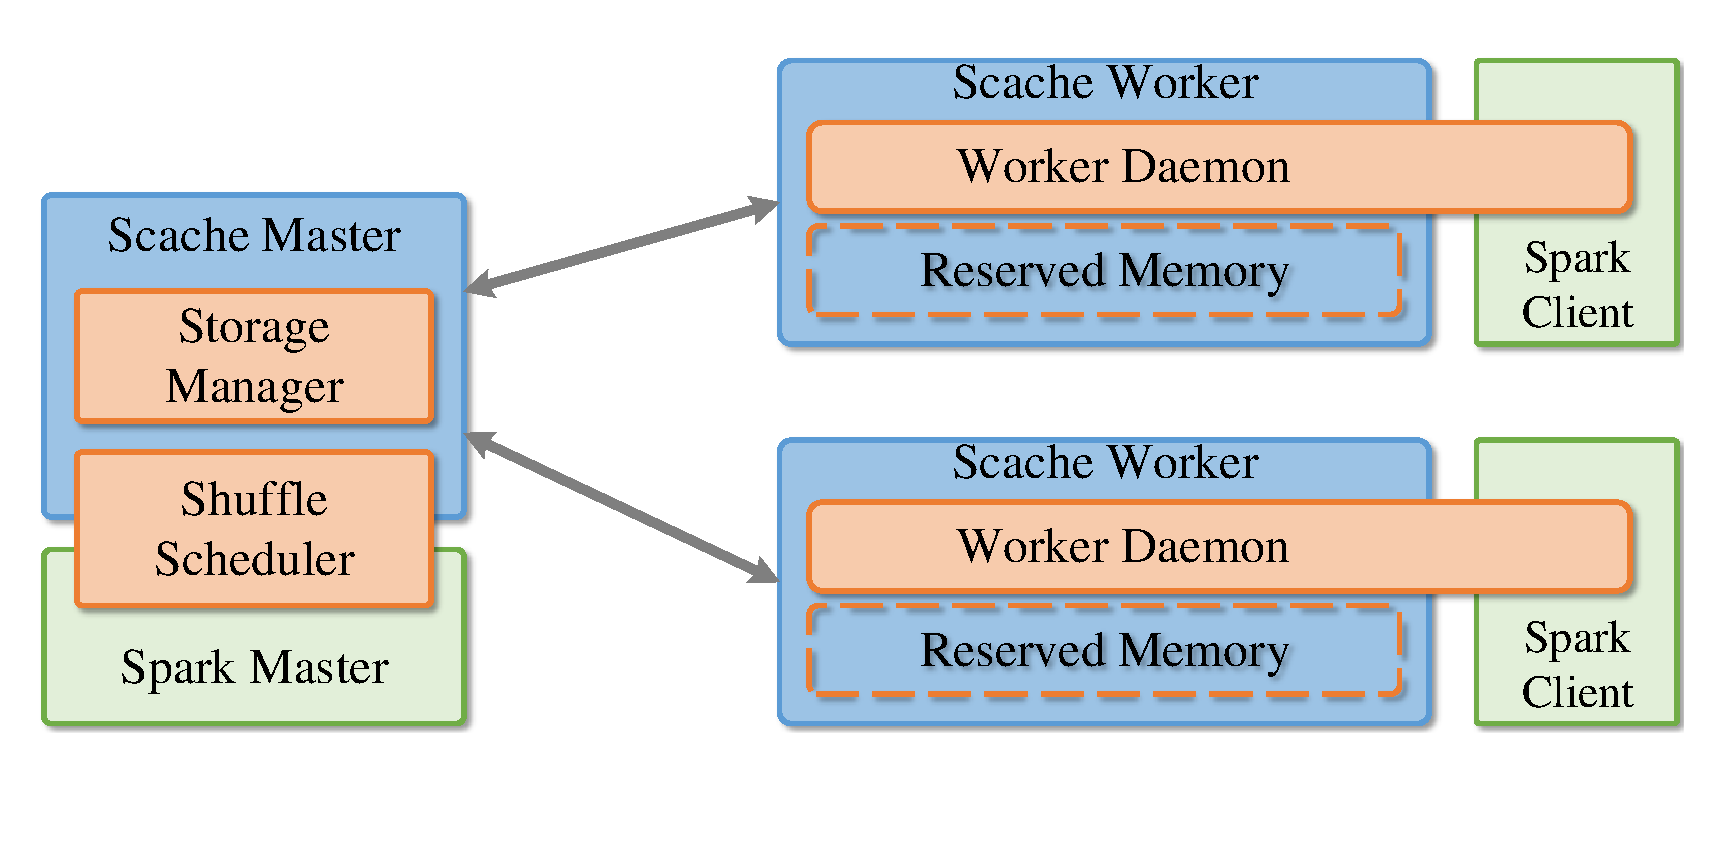
\includegraphics[width=0.8\linewidth]{fig/arch}
	\caption{SCache Architecture}
	\label{fig:arch}
	\vspace{-0.5em}
\end{figure}

\subsection{Memory Management}\label{memorymanage}
As mentioned in Section \ref{observation}, though the shuffle size is relatively small, memory management should still be cautious enough to limit the effect of performance of DAG framework.
When the size of cached blocks reaches the limitation of reserved memory, SCache flushes some of them to the disk temporarily, and re-fetches them when some cached shuffle blocks are consumed or pre-fetched. To achieve the maximum overall improvement, SCache leverages two constraints to manage the in-memory data --- all-or-nothing and context-aware-priority.

\begin{figure}
	\centering
	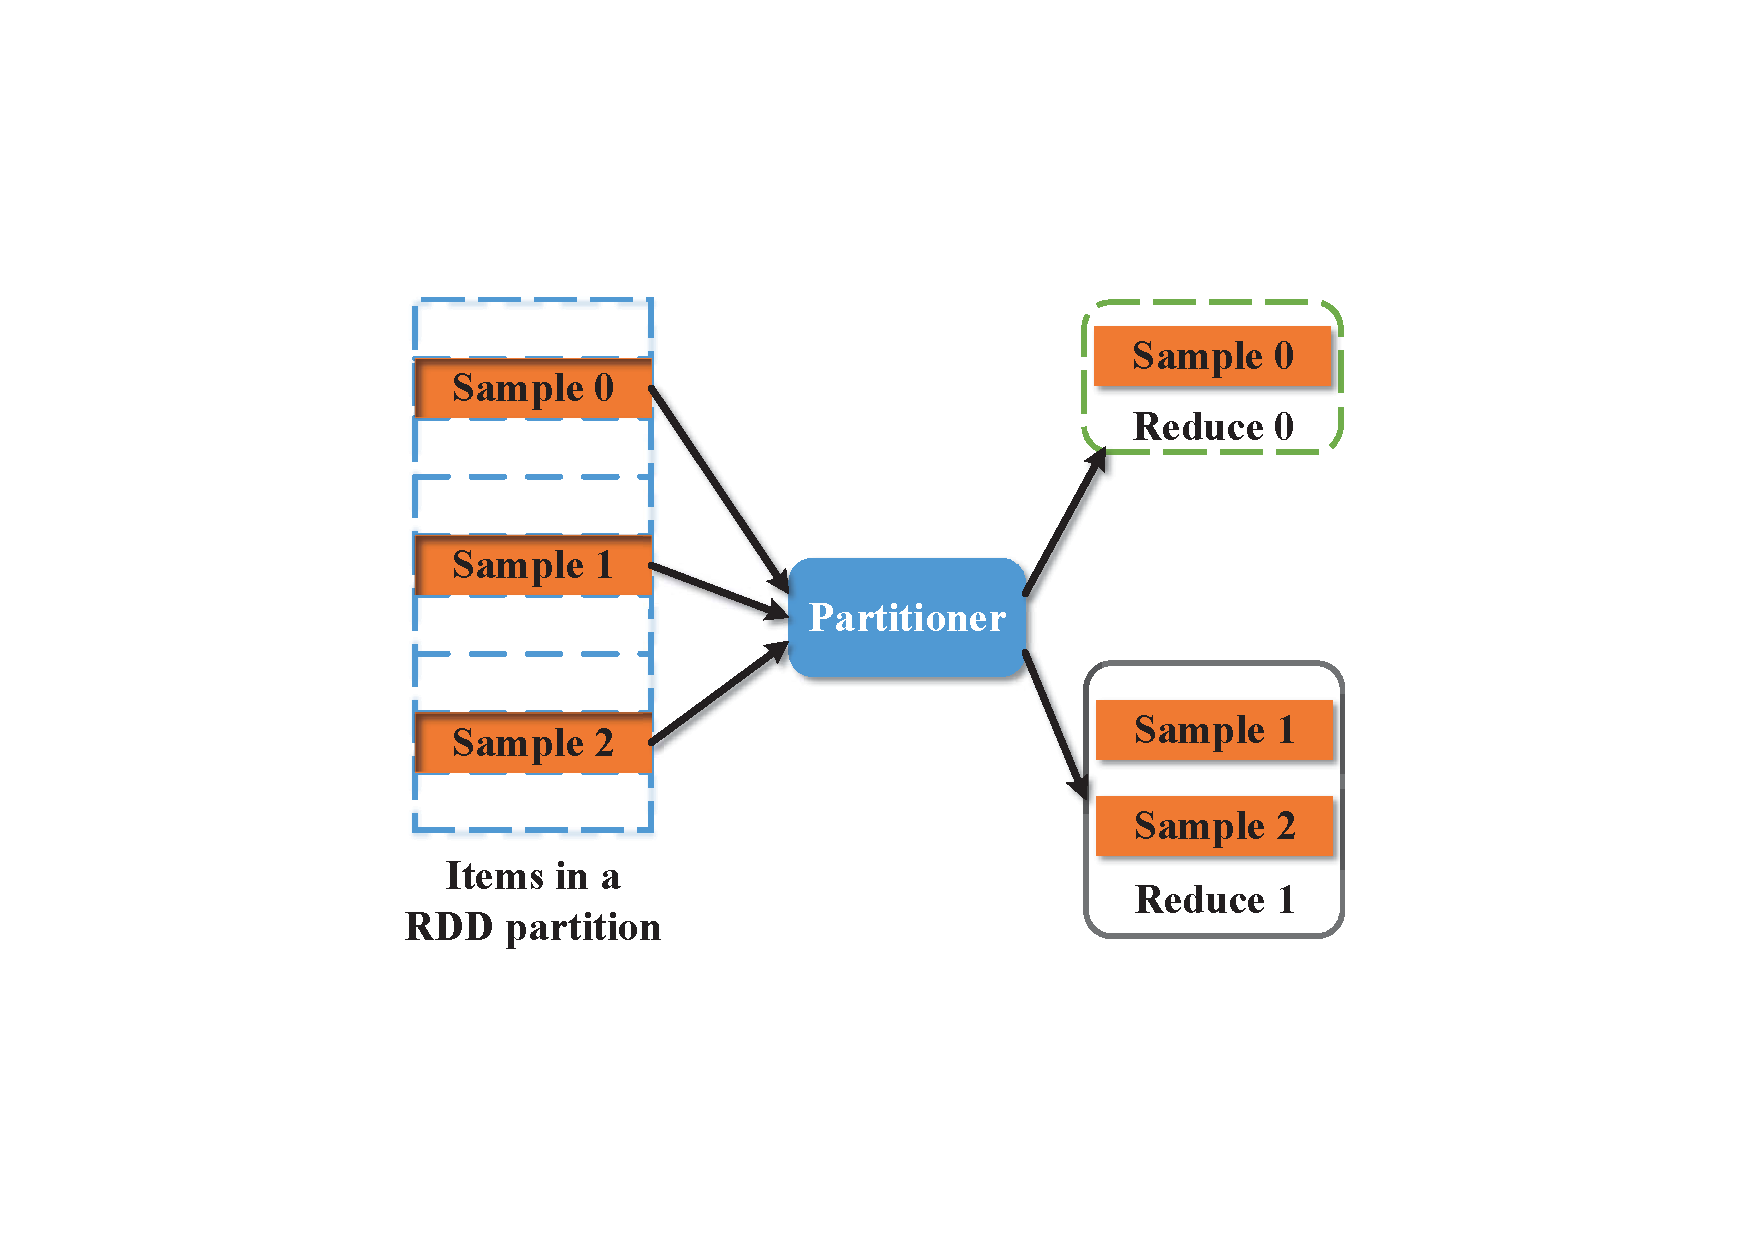
\includegraphics[width=0.6\linewidth]{fig/sample}
	\caption{Reservoir Sampling of One Partition}
	\label{fig:sample}
	\vspace{-1em}
\end{figure}

\subsubsection{All-or-Nothing Constraint}
Memory cached shuffle blocks can speed up the reduce task execution process. But this acceleration of a single task is necessary but insufficient for a shorter stage completion time. Based on the observation in Section \ref{multi}, in most cases one single stage contains multi-rounds of tasks. If one task misses a memory cache and exceeds the original bottleneck of this round, that task might become the new bottleneck and further slow down the whole stage. PACMan \cite{pacman} has also proved that for multi-round stage/job, the completion time improves in steps when $n\times number\ of\ tasks\ in\ one\ round$ of tasks have data cached simultaneously. Therefore, the cached shuffle blocks need to match the demand of all tasks in one running round at least. We refer to this as the all-or-nothing constraint.

According to all-or-nothing constraint, SCache master leverages the pre-scheduled results to determine the bound of each round, and sets corresponding blocks as the minimum unit of storage management.
For those incomplete units, SCache will mark them as the lowest priority.
% Following the all-or-noting constraint can maximum the improvement in stage completion time by using reserved memory efficiently.

\subsubsection{Context-Aware-Priority Constraint}
Unlike the traditional cache replacement schemes such as MIN \cite{min}, the cached shuffle data will only be used once (without failure) in DAG computing. That is, the effort of improving hit rate in most legacy schemes can not benefit DAG application, while their approaches can easily violate the all-or-nothing constraint.
SCache also leverages application context to select victim storage units when the reserved memory is full.

At first, SCache master searches for the incomplete units and flushes all belonging blocks to disk cluster-widely.

If all the units are completed, SCache selects victims based on two factors --- \textit{inter-shuffle units} and \textit{intra-shuffle unit}.
\begin{itemize}[noitemsep]
	\item Inter-shuffle units: SCache master follows the scheduling scheme of Spark to determine the inter-shuffle priority. For a FAIR scheduler, Spark balances the resource among task sets, which leads to a higher priority for those having more tasks unfinished. So SCache sets priorities from high to low in a descending order of remaining storage units of a shuffle unit. For a FIFO scheduler, Spark schedules the task set that is submitted first. So SCache sets the priorities according to the submit time of each shuffle unit.
	\item Intra-shuffle unit: SCache also needs to decide the priority among storage units inside a shuffle unit. According to the task scheduling inside a task set of Spark, the tasks with smaller ID will be scheduled firstly. Based on this, SCache can assign the lower priority to storage units with larger task ID.
\end{itemize}

\subsection{Cost of adapting DAG frameworks}
SCache provides API through RPC, such as \textit{putBlock(blockId)}, \textit{getBlock(blockId)}, and \textit{getScheduleResult(shuffleId)}. The concise design makes it easy to adapt DAG frameworks to enable SCache optimization. For example, it only takes about 500 lines of code in Spark to integrate SCache. By a glance of Hadoop source code, we believe that the costs of enabling SCache on MapReduce \cite{hadoop} and YARN \cite{yarn} based DAG computing framework, such as Tez \cite{tez}, are also very low.

\subsection{Fault tolerance}
Since fault tolerance is not a crucial goal of SCache, we have not implemented fault tolerance mechanism. We plan to implement SCache master with Apache ZooKeeper \cite{zookeeper} to provide constantly service.  For SCache worker, a promising way to prevent failure is to select some backup nodes to store replications of shuffle data during pre-scheduling. In addition, there are also advanced fast recovery techniques such as FineFRC \cite{finefrc}. We leave this to the future work.





% \subsubsection{Fault Tolerance}
% To prevent the machine failure in cluster leading to inconsistency SCache, the master node will log the meta data of shuffle register and scheduling on the disk. Since we remove the shuffle transfer from the critical path of DAG computing, the disk log will not introduce extra overhead to the DAG framworks. Note that the master can be implemented with Apache ZooKeeper \cite{zookeeper} to provide constantly service to DAG framework.
% At the same time, every work node will send a heartbeat to master to report status. If a failure of work node is detected, the master will the do a simple re-schedule. For those scheduled shuffle units, the master assgins the tasks to other workers with more lightweight workload evenly. Then the new assigned worker will fetch the data again. For the incomplete in memory map blocks on the failure node, SCache simply ignore them since DAG framework will schedule the failure map tasks on another node.

\section{Evaluation}\label{evaluation}
\begin{figure}
	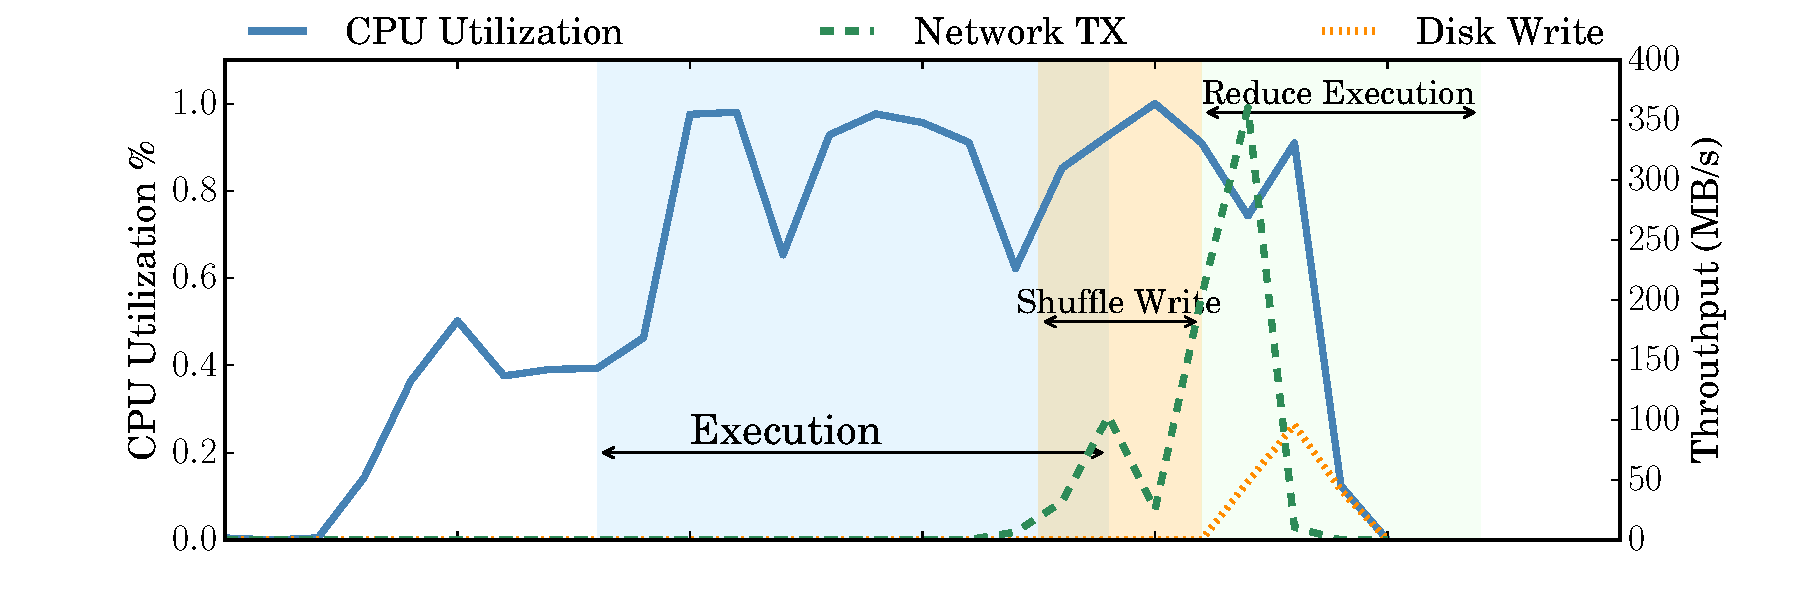
\includegraphics[width=\linewidth]{fig/scache_util}
	\caption{CPU utilization and I/O throughput of a node during a Spark single shuffle application With SCache}
	\label{fig:scache_util}
\end{figure}
In this section, we present the evaluation of SCache with comprehensive workloads and benchmarks. First we run a simple DAG job with single shuffle to analysis hardware utilization and impact of shuffle optimization from the scope of a task to a job. 
Then we use a recognized shuffle intensive benchmark --- Terasort \cite{spark-tera} to evaluate SCache with different data partition schemes.
In order to prove the performance gain of SCache with a real production workload, we also evaluate TPC-DS \cite{sparktpcds} and present the overall performance improvement.
At last, we measure the overhead of weighted reservoir sampling. 
Briefly, SCache can decrease ~$89\%$ time of Spark shuffle. SCache can also achieves a ~$75\%$ and ~$50\%$ improvement of reduce stage completion time respectively in simple DAG application and Terasort without introducing extra network traffic. More impressively, the overall completion time of TPC-DS can be improved ~$40\%$ on average by applying optimization from SCache.
% Because a complex Spark application consists of multiple stages. The completion time of each stage varies under different input data, configurations and different number of stages. This uncertainty leads to the dilemma that dramatic fluctuation occurs in overall performance comparison. To present a straightforward illustration, we limit the scope of most evaluations in a single stage.

\subsection{Setup}\label{stepup}
We implement a Spark demon to enable shuffle optimization as a representative.
We run our experiments on a 50 m4.xlarge nodes cluster on Amazon EC2 \cite{aws}. Each node has 16GB memory and 4 CPUs. The network bandwidth is not specifically provided by Amazon. Our evaluations reveal the bandwidth is about 300 Mbps (see Figure \ref{fig:util}).

\subsection{Simple DAG Analysis}
\subsubsection{Hardware Utilization}
We first run the same single shuffle test (GroupByTest from Spark example \cite{sparksource}) as mentioned in Figure \ref{fig:util}. As shown in Figure \ref{fig:scache_util}, the hardware utilization is captured from one node during the job. Note that since the completion time of whole job is about $50\%$ less than Spark without SCache, the duration of Figure \ref{fig:scache_util} is cut in half as well. An overlap between CPU, disk and network can be easily observed in Figure \ref{fig:scache_util}. That is, the I/O operations will never cut off the computing process with the fine-grained resource allocation. By running Spark with SCache, the overall CPU utilization of the cluster stays in a high level. The decoupling of shuffle write from map tasks frees the CPU earlier and leads to a faster map task computation. The shuffle pre-fetch starting in the early stage of map phase shift the network transfer completion time, so that the computation of reduce can start immediately after scheduled. The combination is the main performance gain we achieved on the scope of hardware utilization by SCache.

\begin{figure}
	%\vspace*{-0.01cm}
	\begin{subfigure}{\linewidth}
		\centering
		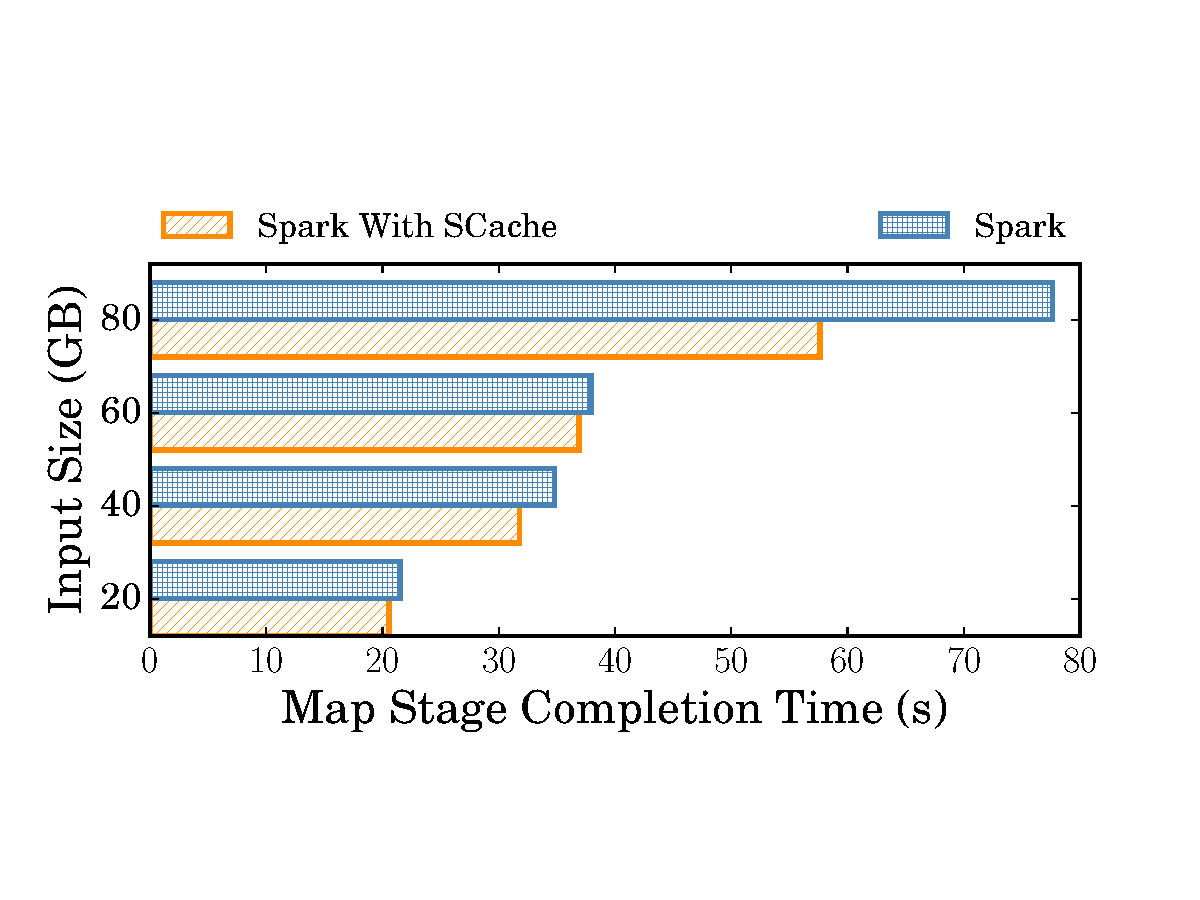
\includegraphics[width=0.9\linewidth]{fig/groupbymapstage}
		\caption{Map Stage Completion Time Comparison}
		\label{fig:mapstage}
	\end{subfigure}
	\begin{subfigure}{\linewidth}
		\centering
		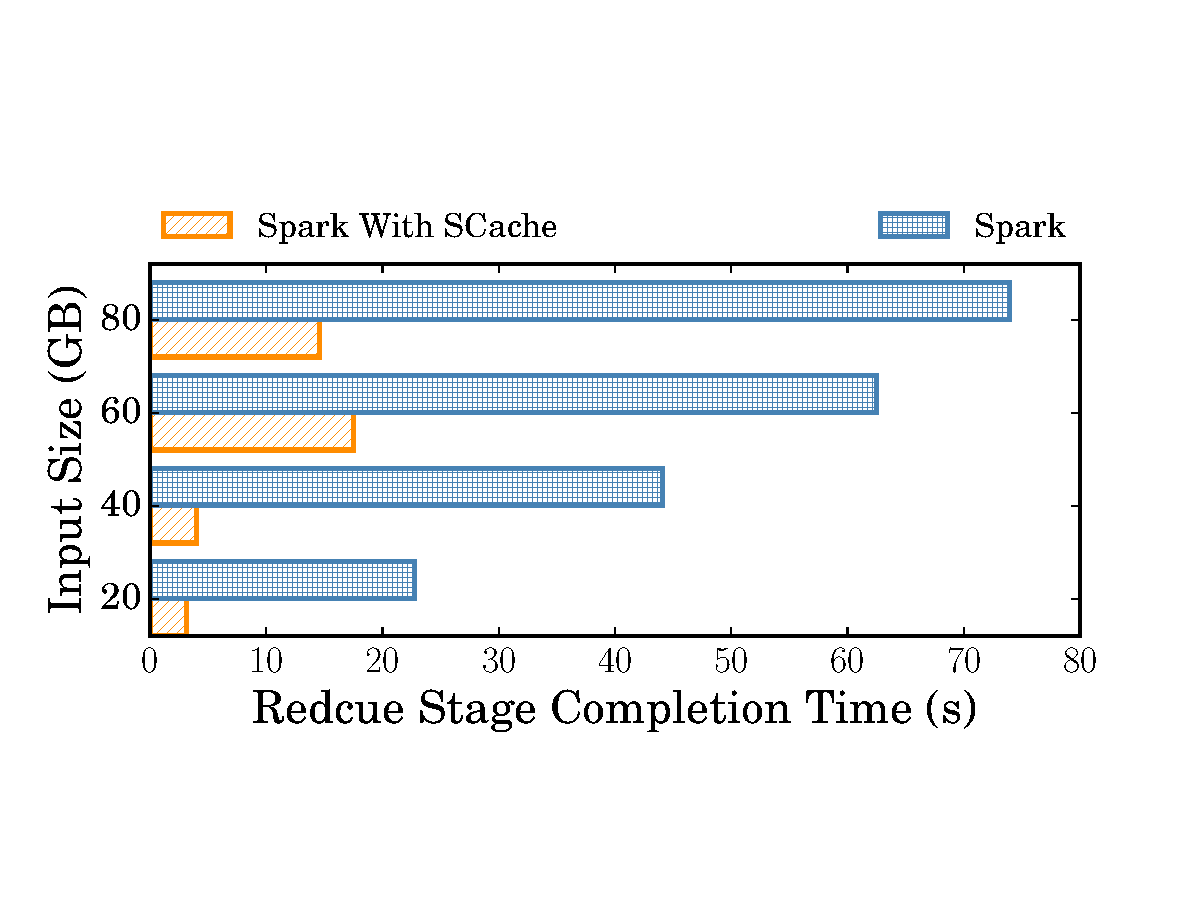
\includegraphics[width=0.9\linewidth]{fig/groupbyreducestage}
		\caption{Reduce Stage Completion Time Comparison}
		\label{fig:reducestage}
	\end{subfigure}
	\caption{Stage Completion Time of Single Shuffle Test}
	\label{fig:singleshuffle}
\end{figure}

\begin{figure}
	\begin{subfigure}{\linewidth}
		\centering
		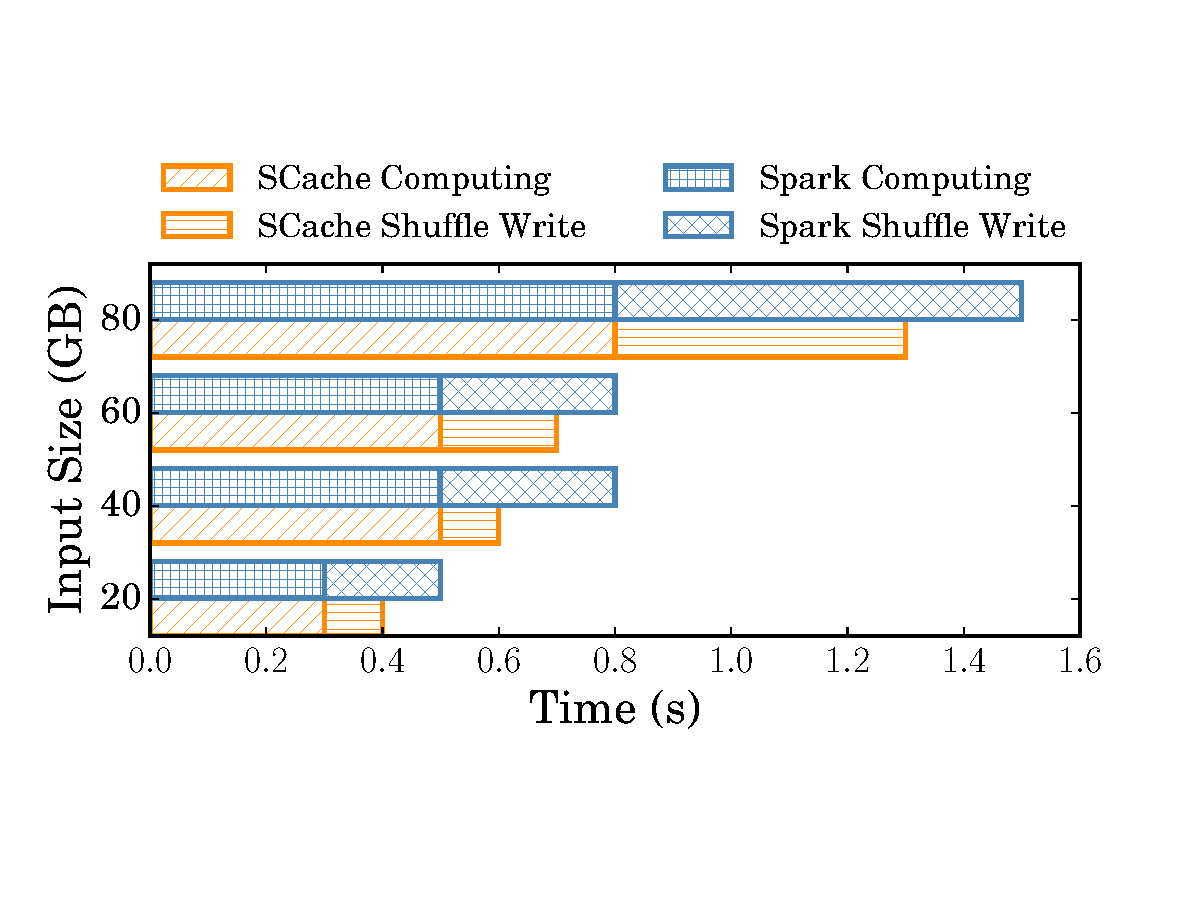
\includegraphics[width=0.9\linewidth]{fig/groupbymaptask}
		\caption{Median Task Details in Map Stages}
		\label{fig:maptask}
	\end{subfigure}
	\begin{subfigure}{\linewidth}
		\centering
		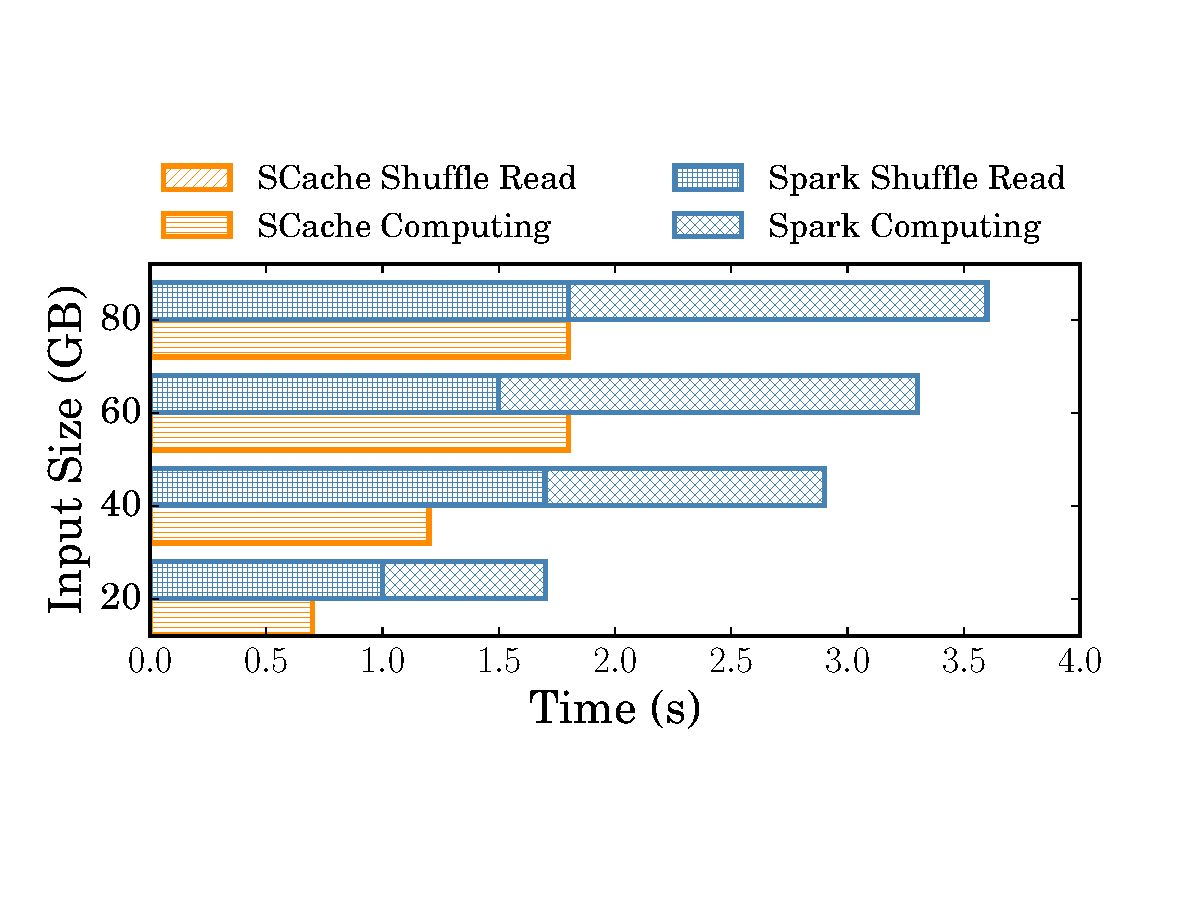
\includegraphics[width=0.9\linewidth]{fig/groupbyreducetask}
		\caption{Median Task Details in Reduce Stages}
		\label{fig:reducetask}
	\end{subfigure}
	\caption{Median Task Completion Time of Single Shuffle Test}
	\label{fig:singleshuffletask}
\end{figure}

The performance is evaluated with different input sizes in the cluster. For each stage, we run 5 rounds of tasks. The stage completion time is presented separately in Figure \ref{fig:mapstage} and Figure \ref{fig:reducestage}. By running spark with SCache, the completion time of map stage can be reduced $10\%$ on average. For reduce stage, instead, SCache achieves a ~$75\%$ performance gain in the completion time of the reduce stage.

A detail analysis into the nutshell of varied overall performance gain on different stages is presented with Figure \ref{fig:singleshuffletask}. For each stage, we pick the median task. About 40\% of shuffle write time can be eliminated by SCache (Figure \ref{fig:maptask}) in a map task. Because the serialization of data is CPU intensive \cite{makingsense} and it is inevitable while moving data out of Java heap memory, SCache can not eliminate the whole phase of shuffle write. This results in a less performance gain in the map stage.
On the reduce side, the network transfer introduces a significantly latency in shuffle read for a single task (Figure \ref{fig:reducetask}). By doing shuffle data pre-fetch for the reduce tasks in Figure \ref{fig:reducetask}, the shuffle read time decreases ~$100\%$, which means shuffle data pre-fetch almost hide all the explicit network transfer in the reduce stage. In overall, SCache can help Spark decreases by ~$89\%$ time in the whole shuffle process. In addition, heuristic reduce tasks scheduling achieves better load balance in cluster than the Spark default FIFO scheduling which may randomly assign two heavy tasks on a single node. So that we can have a significant performance gain in the completion time of the reduce stage.
% \begin{figure*}
% 	\begin{minipage}{\textwidth}
% 		\begin{figure}[H]
% 			\begin{subfigure}{0.5\textwidth}
% 				\centering
% 				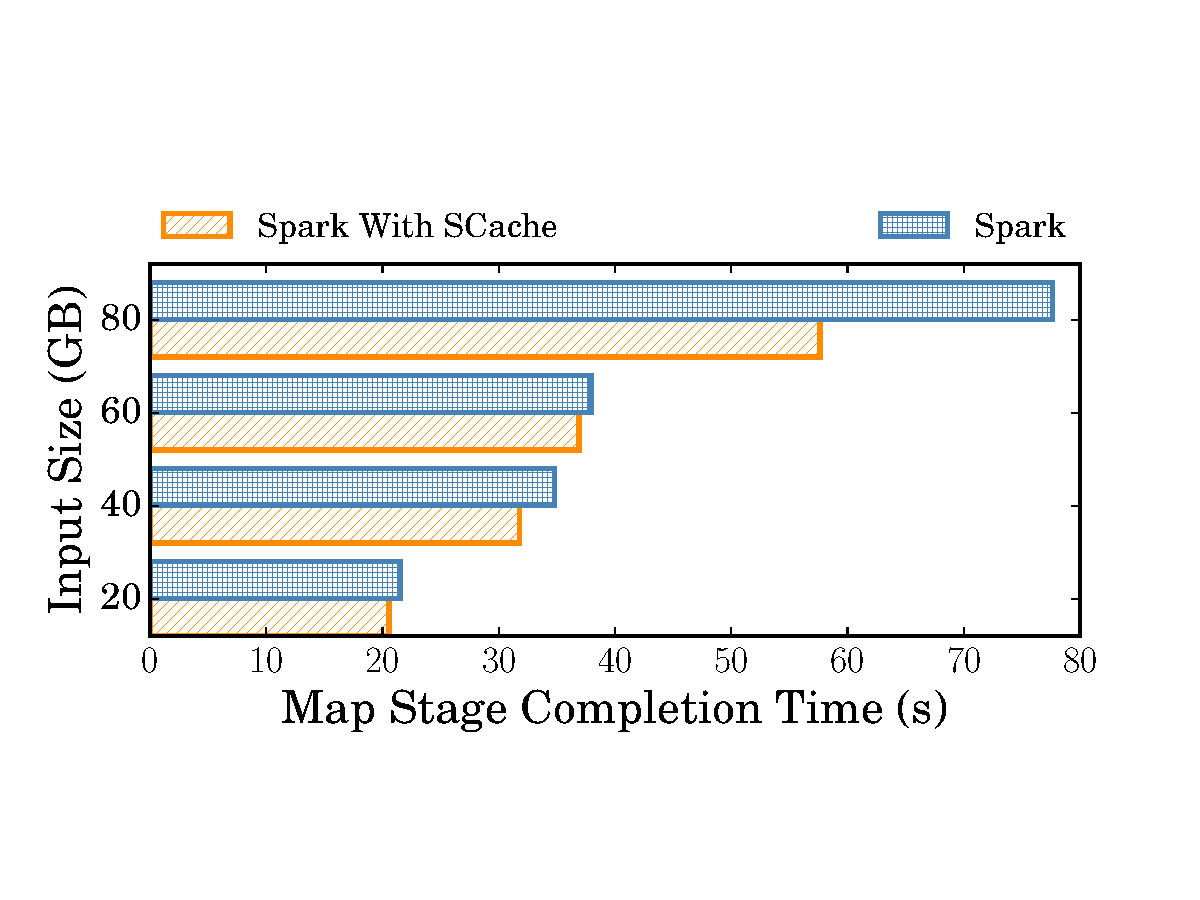
\includegraphics[width=0.8\linewidth]{fig/groupbymapstage}
% 				\caption{Map Stage Completion Time Comparsion}
% 				\label{fig:mapstage}
% 			\end{subfigure}
% 			\begin{subfigure}{0.5\textwidth}
% 				\centering
% 				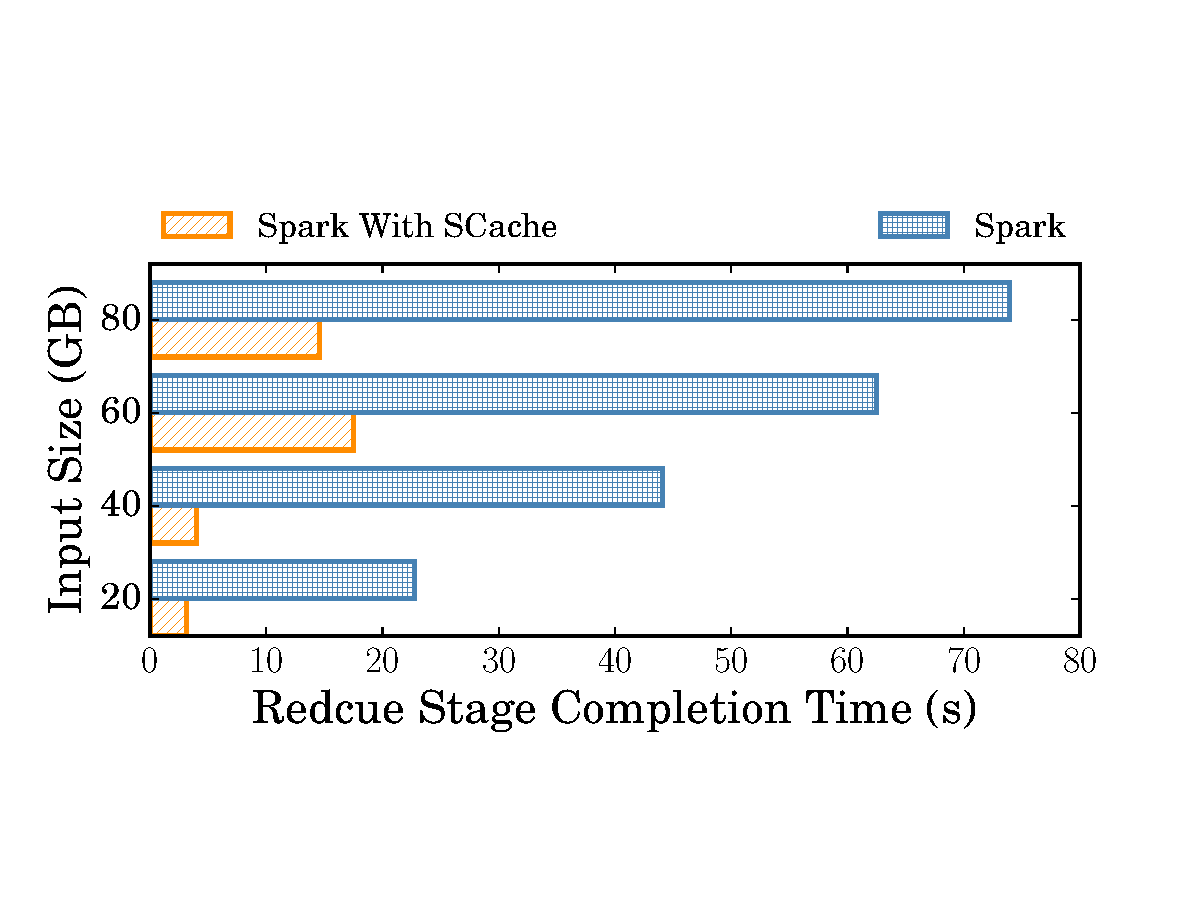
\includegraphics[width=0.8\linewidth]{fig/groupbyreducestage}
% 				\caption{Reduce Stage Completion Time Comparsion}
% 				\label{fig:reducestage}
% 			\end{subfigure}
% 			\caption{Stage Completion Time Comparsion of Single Shuffle Test}
% 			\label{fig:singleshuffle}
% 		\end{figure}
% 	\end{minipage}
% 	\begin{minipage}{\textwidth}
% 		\begin{figure}[H]
% 			\begin{subfigure}{0.5\textwidth}
% 				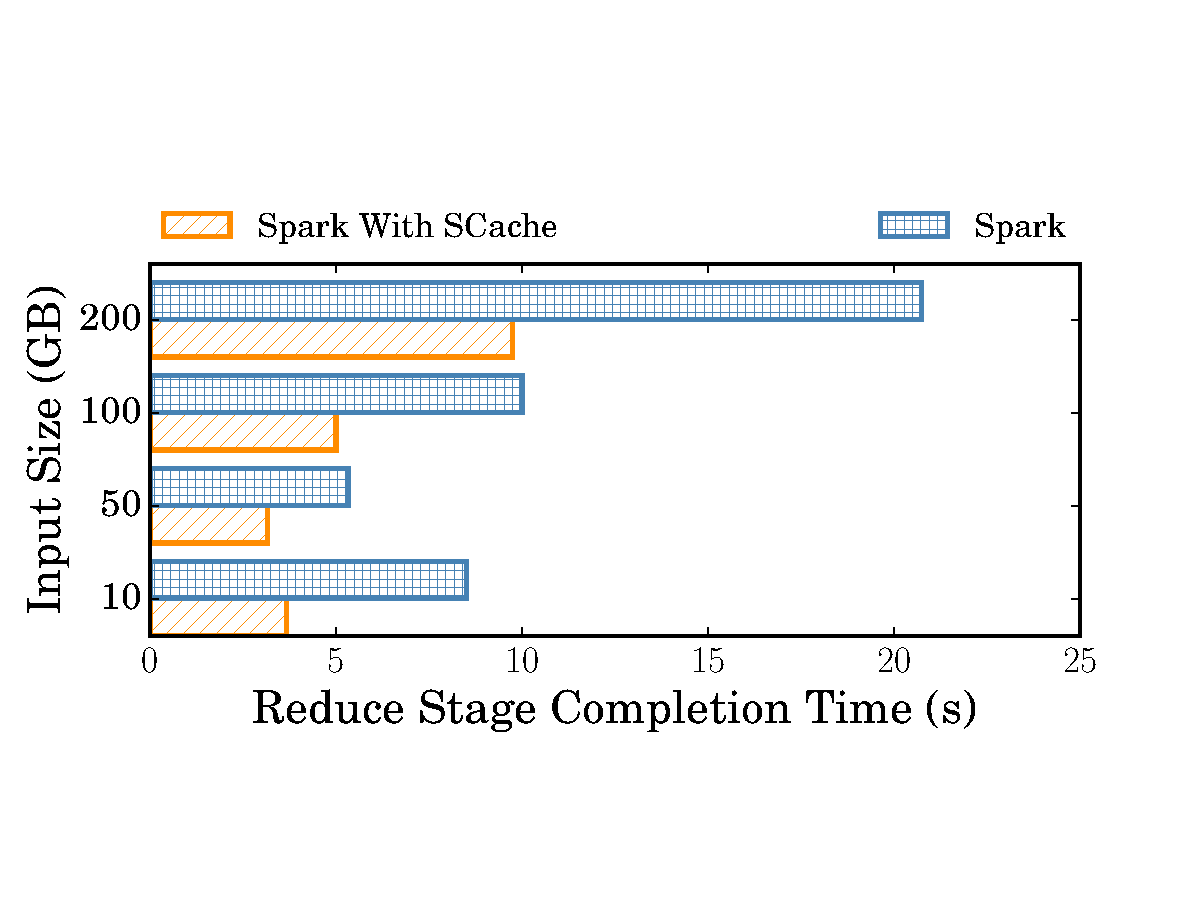
\includegraphics[width=0.8\linewidth]{fig/tera}
% 				\caption{Reduce Stage Completion Time Comparsion}
% 				\label{fig:terasort}
% 			\end{subfigure}
% 			\begin{subfigure}{0.5\textwidth}
% 				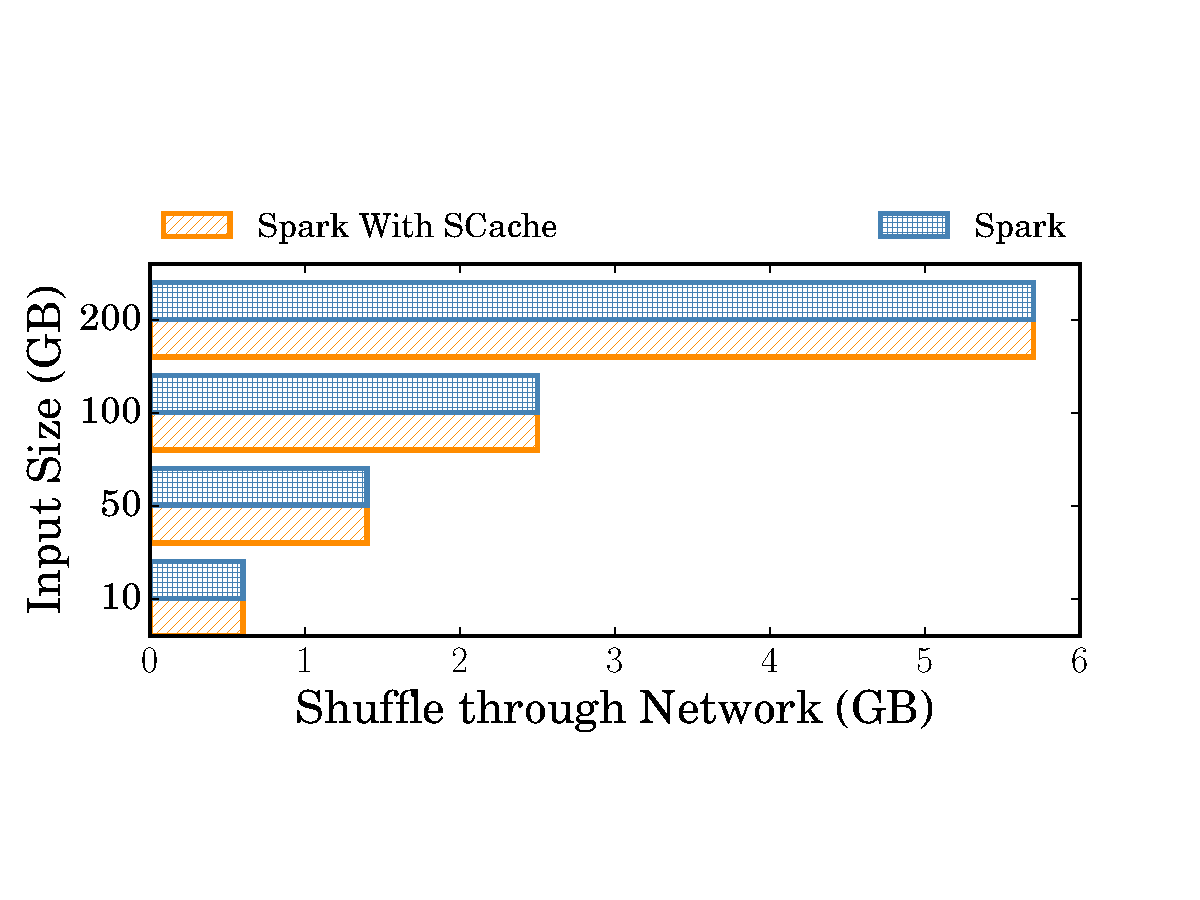
\includegraphics[width=0.8\linewidth]{fig/tera_shuffle}
% 				\caption{Shuffle Data Size Comparsion}
% 				\label{fig:terashuffle}
% 			\end{subfigure}
% 			\caption{Terasort Evaluation}
% 		\end{figure}
		
% 	\end{minipage}
%  \end{figure*}

% \begin{figure}
% \begin{subfigure}{\linewidth}
% 	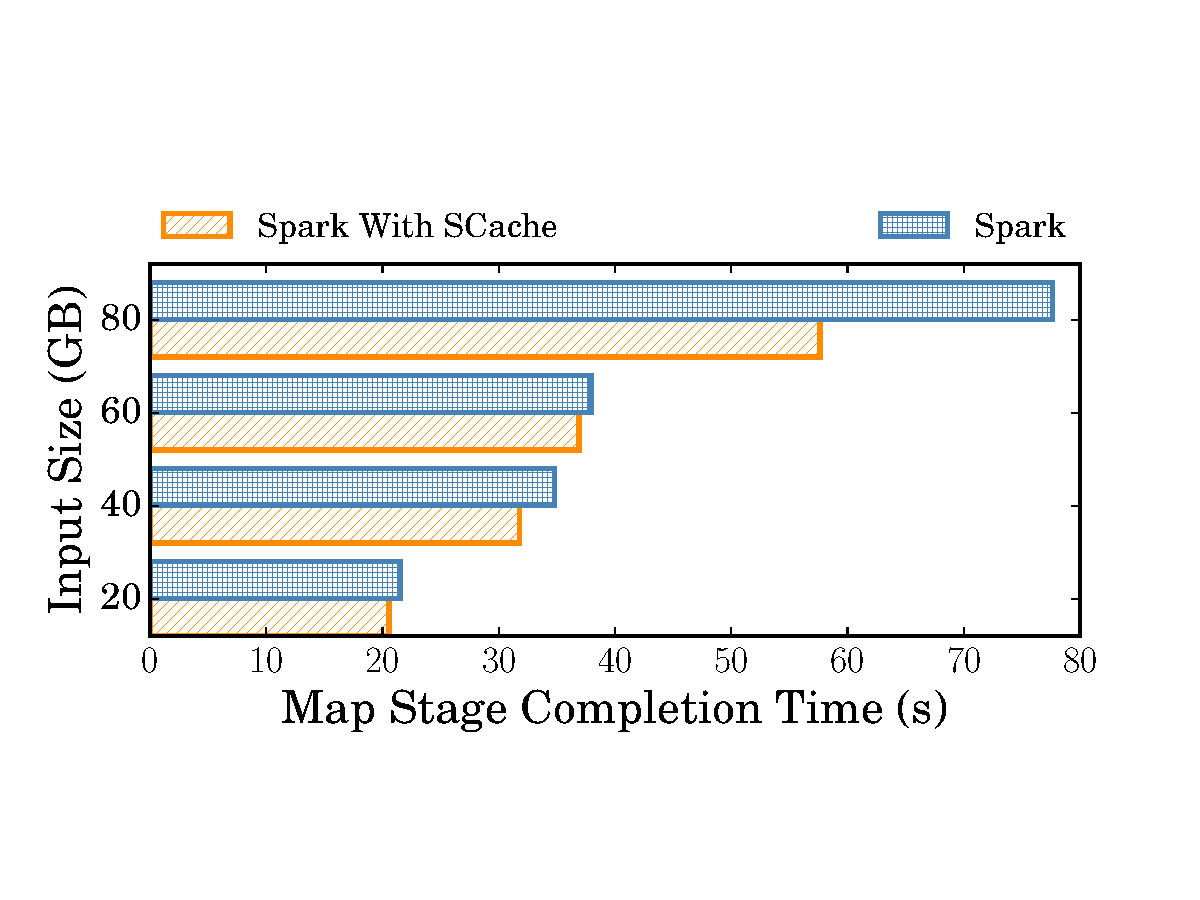
\includegraphics[width=\linewidth]{fig/groupbymapstage}
% 	\caption{Map Stage Completion Time Comparsion}
% 	\label{fig:mapstage}
% \end{subfigure}
% \begin{subfigure}{\linewidth}
% 	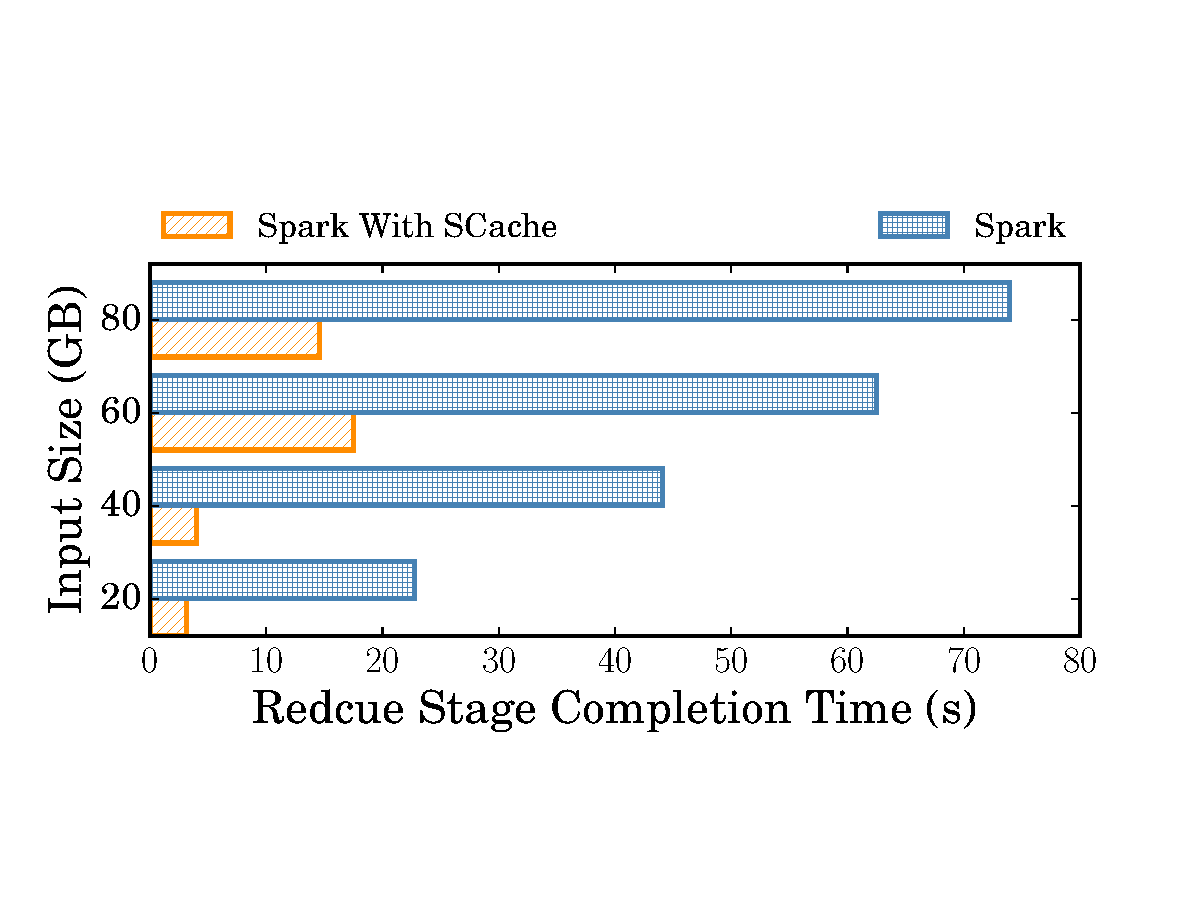
\includegraphics[width=\linewidth]{fig/groupbyreducestage}
% 	\caption{Reduce Stage Completion Time Comparsion}
% 	\label{fig:reducestage}
% \end{subfigure}
% \caption{Stage Completion Time Comparsion of Single Shuffle Test}
% \label{fig:singleshuffle}
% \end{figure}
\subsection{Terasort}
In this part, we evaluate the Terasort \cite{spark-tera}.
Terasort \cite{spark-tera} is a shuffle intensive benchmark for distributed system analysis. It consists of two consecutive shuffles. The first shuffle reads the input data and uses a customized hash partition function for re-partitioning. The second shuffle partitions the data through a range partitioner. As the range bounds set by range partitioner almost match the same pattern of the first shuffle, almost $93\%$ of input data is from one particular map task for each reduce task. It makes the shuffle data transferred through network extremely small under Spark locality preferred task scheduling. So we take the second shuffle as an extreme case to evaluate the scheduling locality for SCache.

As shown in Figure \ref{fig:terasort}, we present the first shuffle as the evaluation of shuffle optimization. At the same time, we use the second the shuffle to evaluate in the dimension of scheduling locality (Figure \ref{fig:terashuffle}). For the first shuffle, Spark with SCache runs 2 $\times$ faster during the reduce stage with the input data in a range from 10GB to 200GB. At the same time, Figure \ref{fig:terashuffle} reveals that SCache pre-scheduling produces exactly same network traffic of second shuffle as Spark, which implies that SCache pre-scheduling can obtain the best locality while balancing the load. In contrast, Spark delays scheduling reduce tasks with the shuffle map output to achieve this optimum.

\subsection{Production Workload}
We also evaluate some shuffle heavy queries from TPC-DS \cite{tpcds}. TPC-DS benchmark is designed for modeling multiple users submitting varied queries (e.g. ad-hoc, interactive OLAP, data mining, etc.). TPC-DS contains 99 queries and is considered as the standardized industry benchmark for testing big data systems. We evaluate the performance of Spark with SCache by picking some of the TPC-DS queries with shuffle intensive attribute. As shown in Figure \ref{fig:tpcds}, on the horizontal axis is query number, and on the vertical axis is query completion time. Spark with SCache outperforms the original Spark in almost all the queries. Furthermore, in many queries, Spark with SCache outperforms original Spark by an order of magnitude. The overall reduction portion of query time that SCache achieved is 40\% on average. Since this evaluation presents the overall job completion time of queries, we believe that our shuffle optimization is promising.
\begin{figure}
	\begin{subfigure}{\linewidth}
		\centering
		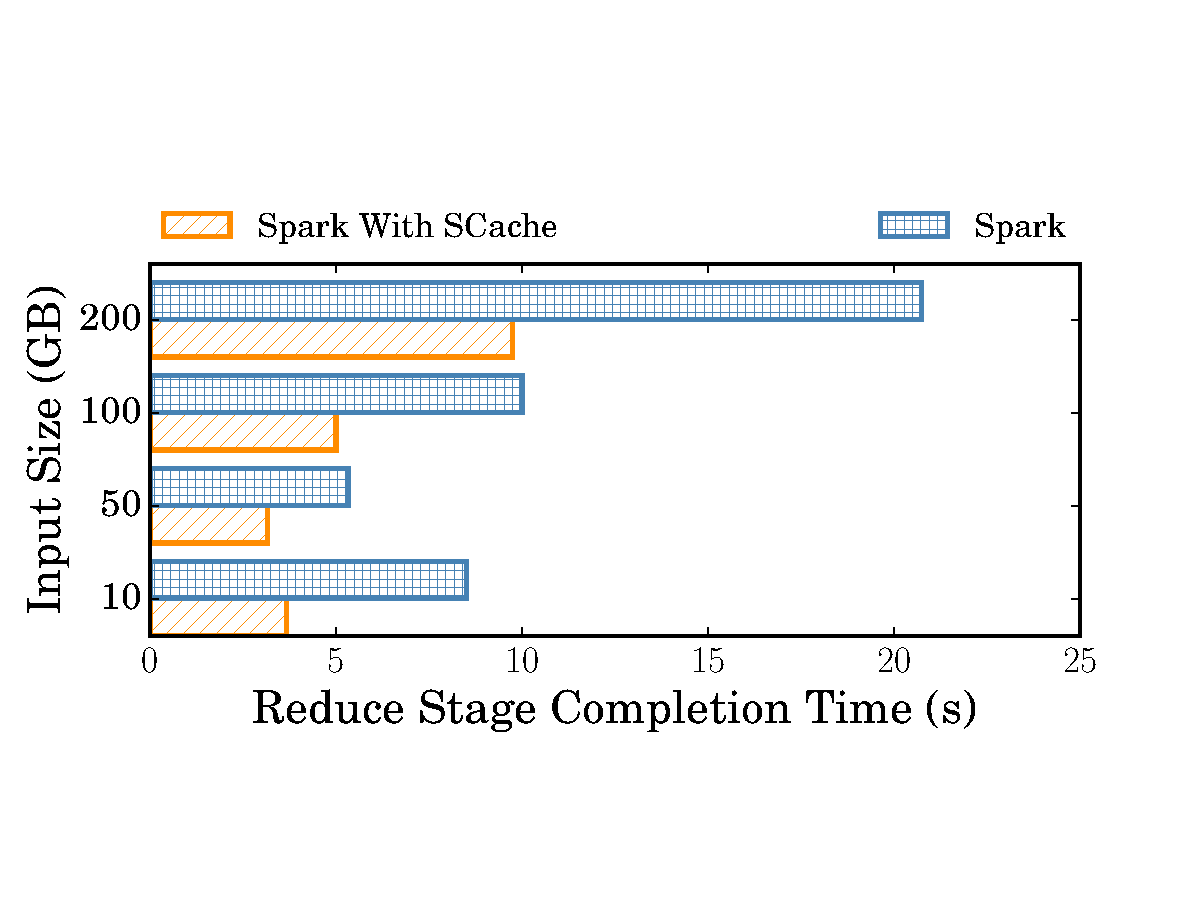
\includegraphics[width=0.915\linewidth]{fig/tera}
		\caption{Reduce Stage Completion Time Comparison of First Shuffle}
		\label{fig:terasort}
	\end{subfigure}
	\vspace{0.08cm}
	\begin{subfigure}{\linewidth}
		\centering
		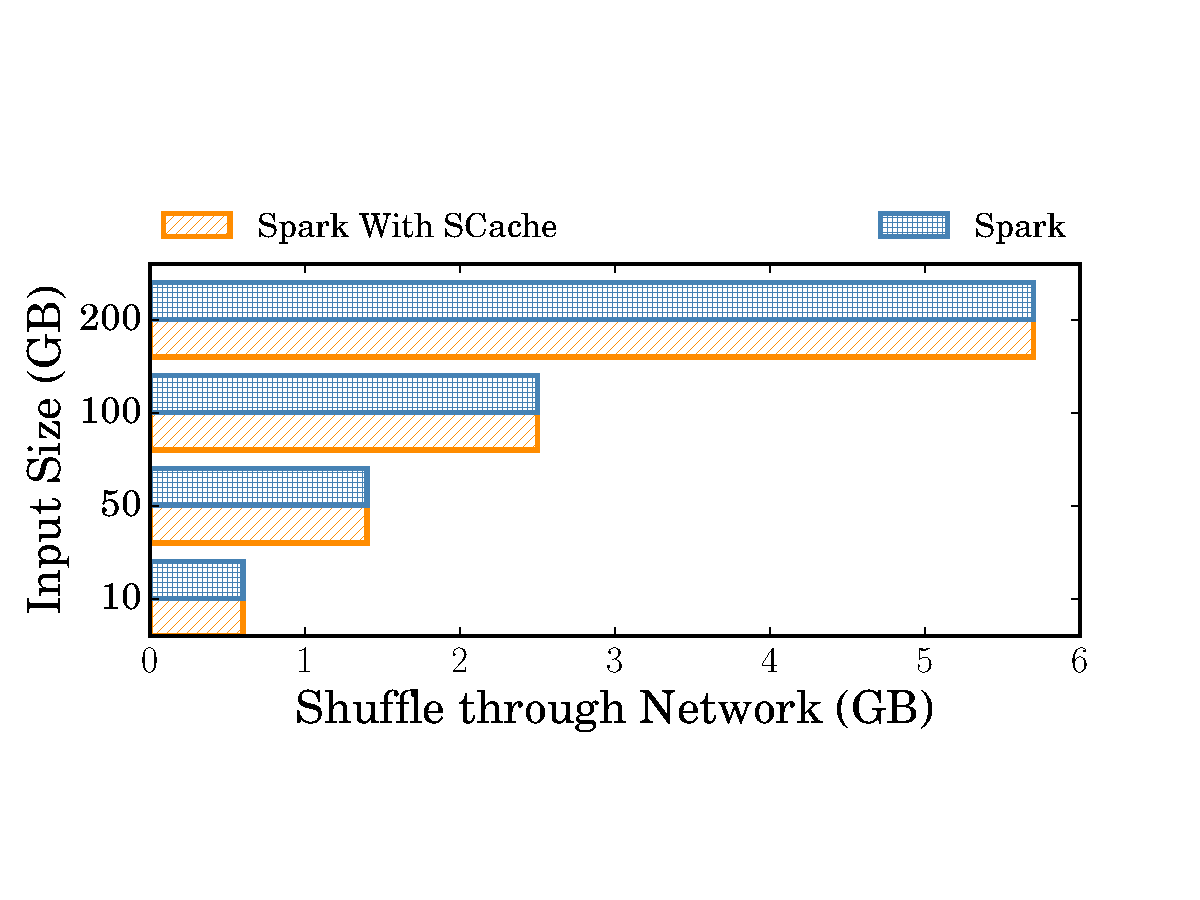
\includegraphics[width=0.915\linewidth]{fig/tera_shuffle}
		\caption{Shuffle Data throuth Network Comparison of Second Shuffle}
		\label{fig:terashuffle}
	\end{subfigure}
	\caption{Terasort Evaluation}
\end{figure}
\subsection{Overhead of Sampling}
In this part, we evaluate the overhead of sampling with different input data sizes on one node and cluster scales. In \ref{fig:sampling}, the overhead of sampling only grows with the increase of input size on each node. But it remains relatively stable when the cluster size scales up. It makes SCache a scalable system in cluster.
\begin{figure*}
	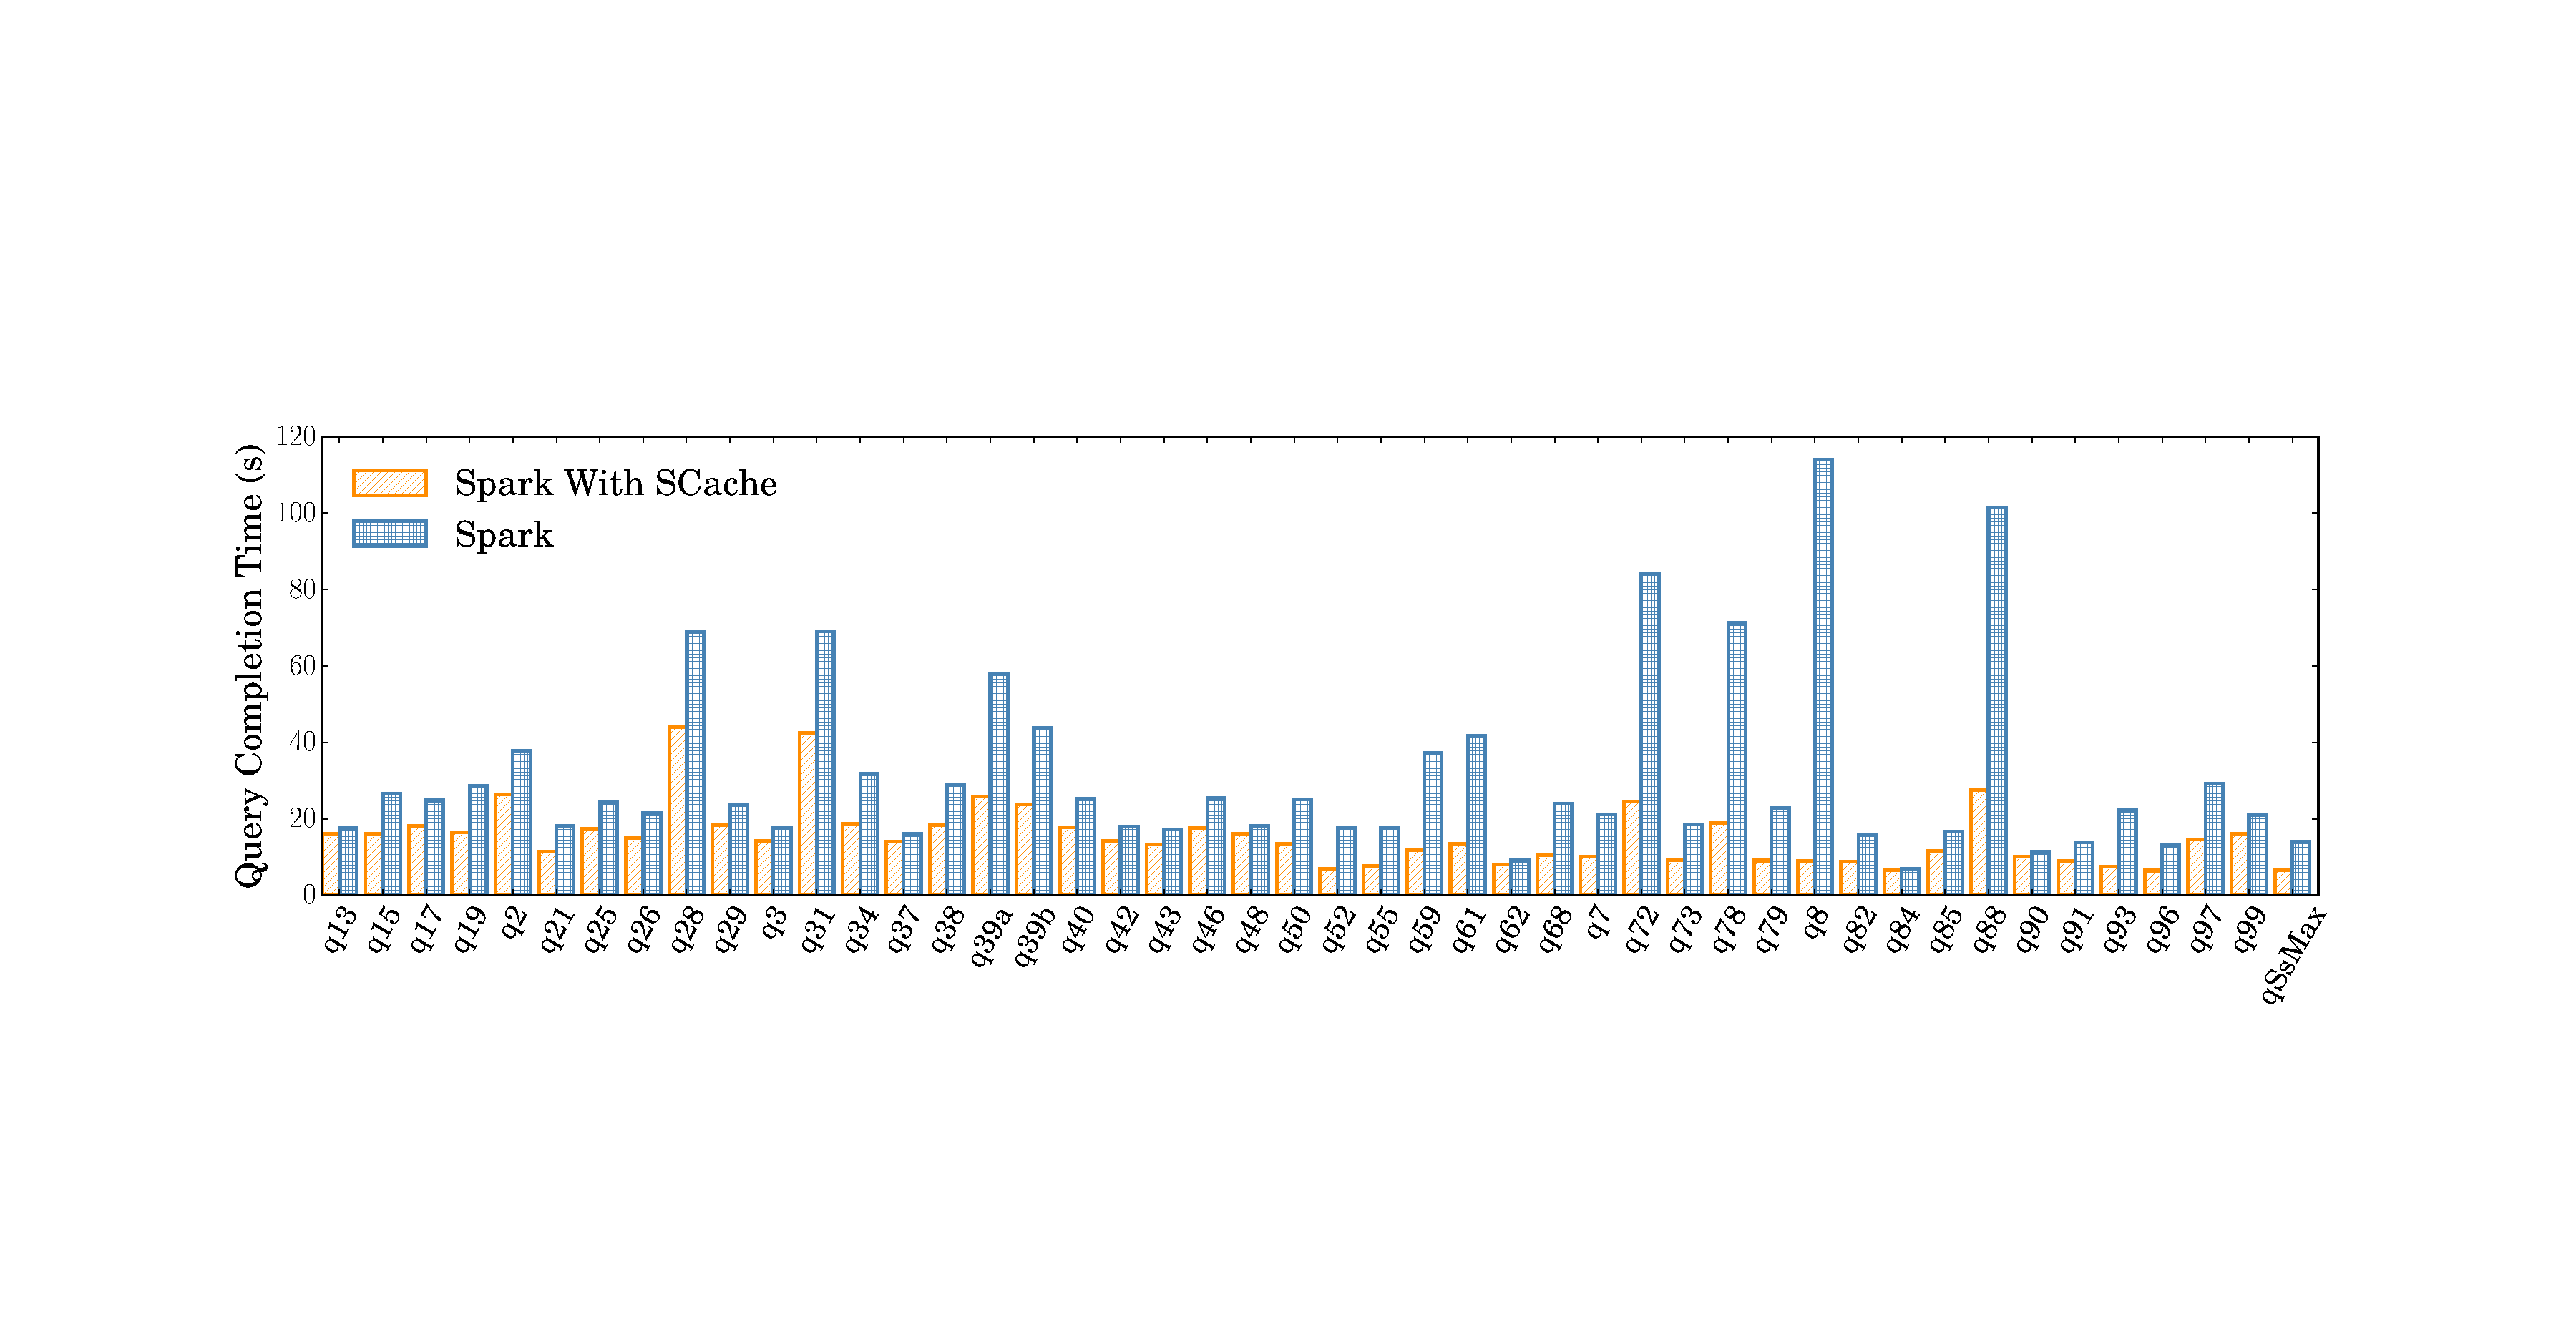
\includegraphics[width=\textwidth]{fig/tpcds}
	\caption{TPC-DS Benchmark Evaluation}
	\label{fig:tpcds}
\end{figure*}



\section{Related Work}
% This section describes related work of shuffle optimization.
\textbf{Pre-scheduling}: Slow-start from Apache Hadoop MapReduce \cite{hadoop} is a classic approach to handle shuffle overhead. 
Starfish \cite{starfish} gets sampled data statics for self-tuning system parameters (e.g. slow-start, etc). 
DynMR \cite{dynmr} dynamically starts reduce tasks in late map stage to decrease the time of shuffle read. 
All of them left the explicit I/O time in an occupied extra slots. 
Instead, SCache starts shuffle pre-fetching without consuming slots. 
iShuffle \cite{ishuffle} decouples shuffle from reducers and designs a centralized shuffle controller. 
But it can neither handle multiple shuffles nor schedule multiple rounds of reduce tasks. 
iHadoop \cite{ihadoop} aggressively pre-schedules tasks in multiple successive stages to start fetching shuffle. 
But we have proved that randomly assign tasks may hurt the overall performance in Section \ref{randomassign}. 
Different from these works, SCache pre-schedules multiple shuffles without breaking load balancing. 
%  by combining DAG information and heuristic algorithms.
\textbf{Delay-scheduling}: Delay Scheduling \cite{delay} delays tasks assignment to get better data locality, which can reduce the network traffic. 
ShuffleWatcher \cite{shufflewatcher} delays shuffle fetching when network is saturated. 
At the same time, it achieves better data locality. 
Both Quincy \cite{quincy} and Fair Scheduling \cite{preemptive} can reduce shuffle data by optimizing data locality of map tasks. 
But all of them can not mitigate explicit I/O in both map and reduce tasks. 
In addition their optimizations fluctuate under different network performances and data distributions, whereas SCache can provide a stable performance gain by shuffle data pre-fetching and in-memory caching.
\textbf{Network layer optimization}: Varys \cite{varys} and Aalo \cite{aalo} provide the network layer optimization for shuffle transfer. 
Though the efforts are limited throughout whole shuffle process, they can be easily applied on SCache to further improve the performance.
%\subsection{Limitation and Future Work}
SCache aims to mitigate shuffle overhead between DAG computing stages. And the evaluation results show a promising improvement. But we realize some limitations of SCache.

\textbf{Fault tolerance of SCache}: When a failure happens on the SCache master, the whole system will stop working. To prevent the inconsistency caused by failure, the master node logs the meta data of shuffle register and pre-scheduling results on the disk. Since we remove the shuffle transfer from the critical path of DAG computing, the disk logging will not introduce extra overhead to the DAG frameworks. Note that the master can be implemented with Apache ZooKeeper \cite{zookeeper} to provide constantly service. If a failure happens on a worker, the optimization of tasks on that node will fail. It also violates the all-or-nothing constraint. A promising way to solve the failure on a worker is to select some backup nodes to store replications of shuffle data during pre-scheduling to prevent the worker failure. In addition, there are also advanced fast recovery techniques such as FineFRC \cite{finefrc}. As for now, fault tolerance is not a crucial goal of SCache,  we leave it to the future work.

%\textbf{Scheduling with different frameworks}: A cluster for data parallel computing always contains more than one frameworks. Setting priority among jobs submitted from different framework is challenging. However, associating with the resource management facilities in data center such as Mesos \cite{mesos} may be a good direction. 

\textbf{Future optimization of Network}: Since the shuffle is decoupled, the network layer optimization, such as Varys \cite{varys} and Aalo \cite{aalo}, can be easily applied on SCache to further improve the performance of shuffle.
\section{Conclusion}
 In this paper, we present SCache, a shuffle optimization scheme for DAG computing framework. SCache decouples the shuffle from computing pipeline and leverages shuffle data pre-fetch to mitigate I/O overhead of the whole system. By scheduling tasks with application context, SCache bridges the gap among computing stages. Our implementation on Spark and evaluations show that SCache can provide a promising speedup to the DAG framework. We believe that SCache is a simple and efficient plugin system to enhance the performance of most DAG computing frameworks.


%% Acknowledgments
%\begin{acks}                            %% acks environment is optional
%                                        %% contents suppressed with 'anonymous'
%  %% Commands \grantsponsor{<sponsorID>}{<name>}{<url>} and
%  %% \grantnum[<url>]{<sponsorID>}{<number>} should be used to
%  %% acknowledge financial support and will be used by metadata
%  %% extraction tools.
%  This material is based upon work supported by the
%  \grantsponsor{GS100000001}{National Science
%    Foundation}{http://dx.doi.org/10.13039/100000001} under Grant
%  No.~\grantnum{GS100000001}{nnnnnnn} and Grant
%  No.~\grantnum{GS100000001}{mmmmmmm}.  Any opinions, findings, and
%  conclusions or recommendations expressed in this material are those
%  of the author and do not necessarily reflect the views of the
%  National Science Foundation.
%\end{acks}


%% Bibliography
%\bibliography{bibfile}
\bibliography{biblio}

%% Appendix
%\appendix
%\section{Appendix}
%
%Text of appendix \ldots

\end{document}
